% Tento soubor nahraďte vlastním souborem s~obsahem práce.
%=========================================================================
% Autoři: Michal Bidlo, Bohuslav Křena, Jaroslav Dytrych, Petr Veigend a~Adam Herout 2019

% Pro kompilaci po částech (viz projekt.tex), nutno odkomentovat a~upravit
%\documentclass[../projekt.tex]{subfiles}
%\begin{document}

\chapter{Úvod}
S~rostoucí digitalizací a~závislostí společnosti na síťové infrastruktuře se problematika efektivní klasifikace síťového provozu stává stále důležitější. Síťový provoz zahrnuje různé typy datových přenosů, jejichž přesné rozlišení hraje klíčovou roli v~oblastech, jako je správa sítí, zajištění bezpečnosti, identifikace anomálií či optimalizace výkonu. Tradiční metody klasifikace, jako jsou \textit{port-based} nebo \textit{payload-based} přístupy, narážejí na limity způsobené šifrováním provozu a~rostoucí složitostí síťových aplikací. Proto se stále více prosazuje využití pokročilých technik strojového učení, které dokážou zpracovávat složitější datové struktury a~přizpůsobovat se dynamickým podmínkám. Zejména metody hlubokého učení nabízejí možnost extrahovat komplexní charakteristiky síťového provozu, které tradiční algoritmy nedokážou efektivně identifikovat. Tyto techniky umožňují analyzovat šifrovaný provoz na základě vnějších vlastností, díky čemuž se strojové učení stává klíčovým nástrojem pro moderní analýzu a~správu sítí.

Tato práce se zaměřuje na aplikaci kontrastivního učení (\textit{contrastive learning}), což je moderní přístup v~oblasti \textit{self-supervised learning}, který umožňuje efektivní učení reprezentací dat bez nutnosti rozsáhlého ručního označování. Hlavní myšlenkou této metody je využití pozitivních a~negativních párů vzorků k~naučení modelu rozlišovat mezi podobnými a~odlišnými charakteristikami dat. V~kontextu klasifikace síťového provozu kontrastivní učení nabízí možnost lepšího porozumění datovým tokům a~zlepšení přesnosti klasifikace zejména u~šifrovaného provozu.

V~rámci kontrastivního učení se v~této práci využívá framework SimCLR (\textit{A Simple Framework for Contrastive Learning of Visual Representations}), který patří mezi moderní a~vysoce efektivní přístupy v~oblasti \textit{self-supervised learning}. Přestože je tento framework primárně navržený pro visuální reprezentace, lze ho využít i~pro síťový provoz. 

V~této práci toho bude docíleno pomocí metody FlowPic, respektive její menší varianty Mini FlowPic. Tento přístup převádí základní data o~síťových tocích do vizuální reprezentace v~podobě histogramu, který se označuje jako FlowPic. Díky tomu je možné využít výhod frameworku SimCLR a~efektivně aplikovat kontrastivní učení. 

Dále si tato práce klade za úkol experimentálně ověřit efektivitu vybraných augmentací síťových toků na různých datových sadách zachycující jak uměle vygenerovaný provoz, tak reálný provoz generovaný lidmi.


%=====================================================================================%
%=====================================================================================%
\chapter{Klasifikace síťového provozu}
Na provoz v~datové síti lze pohlížet jako na tok procházející síťovými prvky. Pro administrativní nebo jiné účely je často zajímavé, užitečné nebo dokonce nezbytné mít přístup k~informacím o~těchto tocích~\cite{rfc7011}. Klasifikace provozu je prvním krokem k~identifikaci a~klasifikaci neznámých tříd síťového provozu. Klasifikace síťového provozu hraje klíčovou roli v~bezpečnosti a~správě sítě, jako je detekce průniků, detekci anomálií, optimalizaci výkonu, ochranu proti škodlivým aktivitám nebo zajištění kvality služby (QoS)~\cite{network_classification}. Díky této technice mohou např. správci sítí přijímat opatření, jako je blokování některých toků, řízení zdrojů či monitorování síťových aplikací.

%=====================================================================================%
\section{Toky síťového provozu}
\label{flows}
V dnešních vysokorychlostních sítích s~přenosovou rychlostí až 100 Gbps vyžaduje pasivní monitorování, jako je zachytávání paketů, nákladný hardware a~rozsáhlou infrastrukturu pro ukládání a~analýzu dat. Efektivnějším a~škálovatelnějším přístupem k~pasivnímu monitorování ve vysokorychlostních sítích je export toků, kdy jsou pakety agregovány do toků a~následně exportovány k~uložení a~analýze~\cite{flow_monitoring}.

RFC 7011 definuje tok jako soubor IP paketů, které procházejí pozorovacím bodem v~síti během určitého časového intervalu, přičemž všechny pakety v~rámci daného toku sdílejí určité společné vlastnosti~\cite{rfc7011}.

V datasetech využívaných v~této práci jsou ony společné vlastnosti ID toku, zdrojová a~cílová IP adresa, zdrojový a~cílový port, protokol, čas prvního a~posledního paketu, počet paketů, jejich směr, velikost a~značka (\textit{label}).

\subsection{Architektura monitorování toků}
Architektura typických systémů pro monitorování toků se skládá z~několika fází. 

První fáze, nazvaná pozorování paketů, zahrnuje zachycení paketů z~pozorovacího bodu a~jejich následné předzpracování. Pozorovacími body mohou být například rozhraní síťových zařízení~\cite{flow_monitoring}.

Druhá fáze se skládá z~procesu měření a~procesu exportu. V~rámci procesu měření jsou pakety seskupovány do toků. Jakmile je tok považován za ukončený, je záznam o~toku exportován prostřednictvím procesu exportu, přičemž záznam je vložen do datagramu podle protokolu pro export toků~\cite{flow_monitoring}.

Třetí fáze je nazvaná sběr dat. Jejím hlavním úkolem je přijímání, ukládání a~předzpracování dat toků generovaných v~předchozí fázi. Mezi běžné operace předzpracování patří agregace, filtrování, komprese dat a~vytváření souhrnů~\cite{flow_monitoring}.

Poslední fází je analýza dat. V~rámci výzkumných nasazení má analýza dat často průzkumný charakter (tj. manuální analýza), zatímco v~operačních prostředích jsou analytické funkce obvykle integrovány do fáze sběru dat (tj. kombinace manuální a~automatizované analýzy). Mezi běžné analytické činnosti patří korelace a~agregace, profilování, klasifikace a~charakterizace provozu, detekce anomálií a~identifikace průniků~\cite{flow_monitoring}.
\begin{figure}[H]
	\centering
	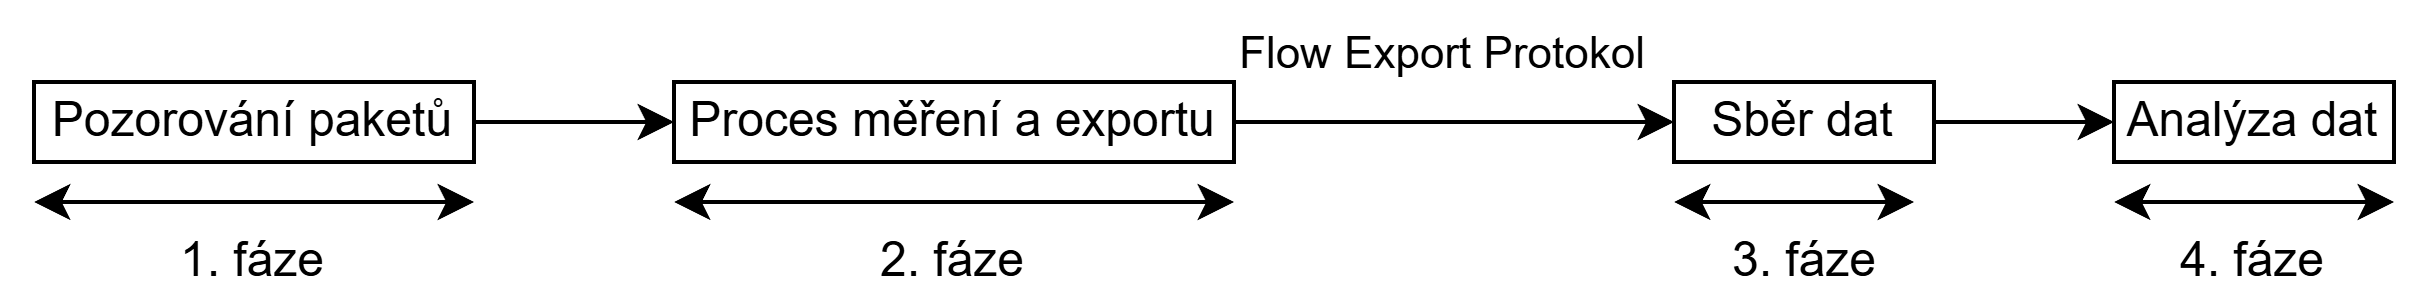
\includegraphics[width=1\textwidth]{obrazky-figures/good_flow_monitoring.png}
	\caption{Architektura typické sestavy pro monitorování toků~\cite{flow_monitoring}.}
	\label{flow_monitoring}
\end{figure}


Dva hlavní protokoly pro export toků jsou NetFlow~\cite{rfc3954} a~Internet Protocol Flow Information Export (IPFIX)~\cite{rfc7011}.

%mozna popsat vice do teorie, nez jeh historii.
\subsection{NetFlow}
V devadesátých letech dvacátého století začala společnost Cisco pracovat na vlastní technologii exportu toků, kterou pojmenovala NetFlow. Tuto technologii firma patentovala v~roce 1996. Zpočátku se jednalo o~proprietární protokol, který byl kompatibilní pouze se zařízeními Cisco. První verze, která získala široké rozšíření, byla NetFlow v5, která byla veřejnosti zpřístupněna kolem roku 2002 a~popsána v~RFC 3954~\cite{rfc3954}. Nejnovější verzí NetFlow je NetFlow v9, která byla představena v~roce 2004.

\subsection{IPFIX}
V devadesátých letech dvacátého století standardizovala \textit{Internet Engineering Task Force} (IETF) protokol \textit{Realtime Traffic Flow Management} (RTFM), sloužící k~měření síťových toků na základě SNMP\footnote{\url{https://doi.org/10.17487/RFC1157}}. V~roce 2001 zahájila IETF iniciativu zaměřenou na vytvoření interoperabilního protokolu pro export síťových toků v~rámci pracovní skupiny IPFIX. Výsledkem tohoto úsilí byla definice požadavků (RFC 3917~\cite{rfc3917}) a~následné zhodnocení kandidátních protokolů (RFC 3955~\cite{rfc3955}) vhodných pro měření síťových toků, jak bylo detailně popsáno v~prohlášení o~použitelnosti IPFIX (RFC 5472~\cite{rfc5472}). Pracovní skupina, s~cílem vycházet při návrhu budoucího standardu co nejvíce z~existujících de facto standardů, zvolila jako základ protokol Cisco NetFlow v9~\cite{rfc3954}. Tento protokol, nástupce široce používaného NetFlow v5, byl vytvořen s~ohledem na specifické požadavky stanovené IPFIX~\cite{IPFIX}.

IPFIX definuje architekturu (RFC 5470~\cite{rfc5470}), která představuje zobecnění existujících architektur používaných v~měřicích infrastrukturách. Tato architektura poskytuje jednotnou terminologii a~formuluje předpoklady na architektonické úrovni, které protokol předpokládá.

Architektura rozlišuje tři základní typy procesů: měřicí procesy (MPs), jež generují toky na základě pozorovaných paketů, exportní procesy (EPs), které zajišťují přenos toků prostřednictvím protokolu IPFIX do sběrných procesů (CPs). Všechny vztahy mezi těmito procesy mají charakter jednoho vůči mnoha, například exportní proces může exportovat toky z~více měřicích procesů do několika sběrných procesů, přičemž každý sběrný proces může přijímat IPFIX zprávy od více exportních procesů a~naopak.

Snahy o~škálování IPFIX pro rozsáhlá a~vícevrstvá nasazení vedly k~zavedení intermediárních procesů (ImPs), které provádějí úpravy toků, jako je jejich agregace, korelace či anonymizace. Zařízení, které kombinuje sběrný proces, jeden nebo více intermediárních procesů a~exportní proces, se označuje jako mediátor~\cite{IPFIX}.

%=====================================================================================%
\section{Metody klasifikace síťového provozu}
Klasifikace síťového provozu je proces identifikace síťových aplikací nebo protokolů, které se vyskytují v~síti. Existuje mnoho různých metod pro klasifikaci síťových aplikací, nicméně tato práce se se zaměří na tři hlavní přístupy:  klasifikace založená na portech (tzv. \textit{Port-based Classification}), klasifikace založená na datech přenášených v~paketech (tzv. \textit{Payload-Based Classification}) a~nakonec klasifikace pomocí strojového učení (ML)~\cite{network_classification}.

\subsection{Port-based klasifikace}
\label{port_based}
Klasifikace síťových aplikací se provádí pomocí tzv. \textit{well-known} čísel portů. Provoz je identifikován na základě portů registrovaných u~\textit{Internet Assigned Numbers Authority} (IANA\footnote{\url{https://www.iana.org/}}). Například e-mailové aplikace používají port 25 (SMTP\footnote{\url{https://doi.org/10.17487/RFC5321}}) pro odesílání e-mailů a~port 110 (POP3\footnote{\url{https://doi.org/10.17487/RFC1939}}) pro jejich přijímání. Dalším známým příkladem jsou webové aplikace, které využívají port 80. Tento přístup však neposkytuje příliš přesné výsledky klasifikace~\cite{network_applications}. Tato technika navíc selhává kvůli používání dynamických čísel portů nových aplikací, aby se vyhnula odhalení~\cite{network_classification}.

\subsection{Payload-based klasifikace}
Tato metoda, známá jako technika hluboké analýzy paketů (\textit{Deep Packet Inspection}, DPI), spočívá v~prozkoumání obsahu paketů a~hledání charakteristických signatur síťových aplikací v~síťovém provozu. Je to první alternativa k~metodě založené na portech zmíněné~v~\ref{port_based}. Tato technika je zvláště určena pro aplikace typu \textit{Peer to Peer} (P2P), které používají dynamická čísla portů~\cite{transport_layer_id}.

Tato technika má však několik nedostatků. Prvním problémem je, že vyžaduje nákladný hardware pro vyhledávání vzorců v~datech paketů. Druhým problémem je, že ji nelze použít u~šifrovaného síťového provozu. Kromě toho tento přístup vyžaduje neustálé aktualizace signaturních vzorců pro nové aplikace~\cite{network_classification}.

\subsection{Klasifikace pomocí strojového učení}
Technika strojového učení (ML) spočívá v~analýze a~učení vzorců z~již zachyceného síťového provozu. V~rámci této metody se klasifikátor strojového učení trénuje na základě tréninkových vzorků, a~poté se pomocí tohoto modelu klasifikují neznámé třídy~\cite{network_classification}. V~této práci se právě tato metoda klasifikace síťového provozu využívá. Konkrétně se jedná o~kontrastní učení, které je popsáno v~sekci~\ref{contrastive_learning}.

%=====================================================================================%
\section{Klasifikace šifrovaného síťového provozu}
S rychlým růstem objemu internetového provozu se bezpečnost síťových spojení stává klíčovým aspektem, jelikož prostřednictvím internetu dochází k~přenosu velkého množství citlivých uživatelských informací, jako jsou například bankovní údaje a~záznamy o~platbách. Pro zajištění důvěrnosti a~integrity dat se široce implementují moderní šifrovací technologie jako je \textit{Secure Socket Layer/Transport Layer Security} (SSL/TLS)\footnote{\url{https://doi.org/10.17487/RFC8446}}, které poskytují nezbytnou ochranu síťových spojení. Avšak neustálý nárůst šifrovaného provozu přináší nové výzvy pro analýzu síťového provozu. Tradiční metody, které se při analýze spoléhaly na přístup k~obsahu nešifrovaných paketů (\textit{plaintext payload}), v~případě šifrovaného provozu ztrácejí svou efektivitu, neboť tento obsah již není dostupný~\cite{encrypted_traffic}.

\subsection{Feature-based metody}
Jedním z~přístupů ke klasifikaci šifrovaného síťového provozu jsou metody založené na vlastnostech síťového provozu (\textit{feature-based}). Tyto metody se nezaměřují na obsah datových částí paketů, ale na vnější charakteristiky síťového provozu, jako jsou velikost paketů, časové intervaly mezi jejich přenosy, počet paketů v~obou směrech komunikace a~doba trvání síťového spojení. Tyto charakteristiky zůstávají do určité míry stabilní i~v~případě šifrované komunikace, což umožňuje efektivní analýzu a~klasifikaci provozu~\cite{survey_enc_traffic}.

Některé dodatečné informace je možné získat také během inicializační fáze šifrovaných protokolů. Typickým příkladem je \textit{TLS handshake}, který často obsahuje nešifrované části umožňující analýzu. Tato fáze může poskytnout cenné informace o~šifrovacích algoritmech a~dalších parametrech použitého protokolu, což je užitečné pro identifikaci typu šifrované komunikace.

\subsection{FlowPic}
\label{flowpic_text}
Další metodou pro klasifikaci šifrovaného internetového provozu a~identifikaci aplikací je FlowPic. Tento přístup převádí základní data o~síťových tocích, kteté jsou popsány v~sekci~\ref{flows}, do vizuální reprezentace v~podobě obrazu, označovaného jako FlowPic, a~následně aplikuje pokročilé techniky hlubokého učení, konkrétně konvoluční neuronové sítě (CNNs), které jsou popsány v~sekci~\ref{CNNs}, k~určení kategorie síťového toku (např. prohlížení webu, chat, streamování videa) a~identifikace konkrétní aplikace, která daný tok generuje~\cite{FlowPic}.

FlowPic vytváří obraz založený na dvourozměrném histogramu síťového toku. Tento obraz lze chápat jako pole distribucí velikostí datových částí paketů (\textit{Payload Size Distributions}, PSD), kde každá PSD odpovídá specifickému časovému intervalu v~rámci jednosměrného síťového toku. Vzhledem k~tomu, že naprostá většina velikostí paketů nepřesahuje 1\,500 bajtů (hodnota maximální přenosové jednotky (MTU) pro Ethernet), pakety s~velikostí větší než 1\,500 bajtů jsou ignorovány a~osa $Y$ je omezena na rozsah 1 až 1\,500 bajtů~\cite{FlowPic_classification}.  

Následně jsou všechny normalizované páry vloženy do dvourozměrného histogramu, kde každá buňka obsahuje počet paketů, které dorazily v~daném časovém intervalu a~mají odpovídající velikost. Každý histogram o~rozměrech 1\,500$\times$1\,500 je uložen jako maticová reprezentace obrazu, která se nazývá FlowPic~\cite{FlowPic_classification}.
\begin{figure}[H]
	\centering
	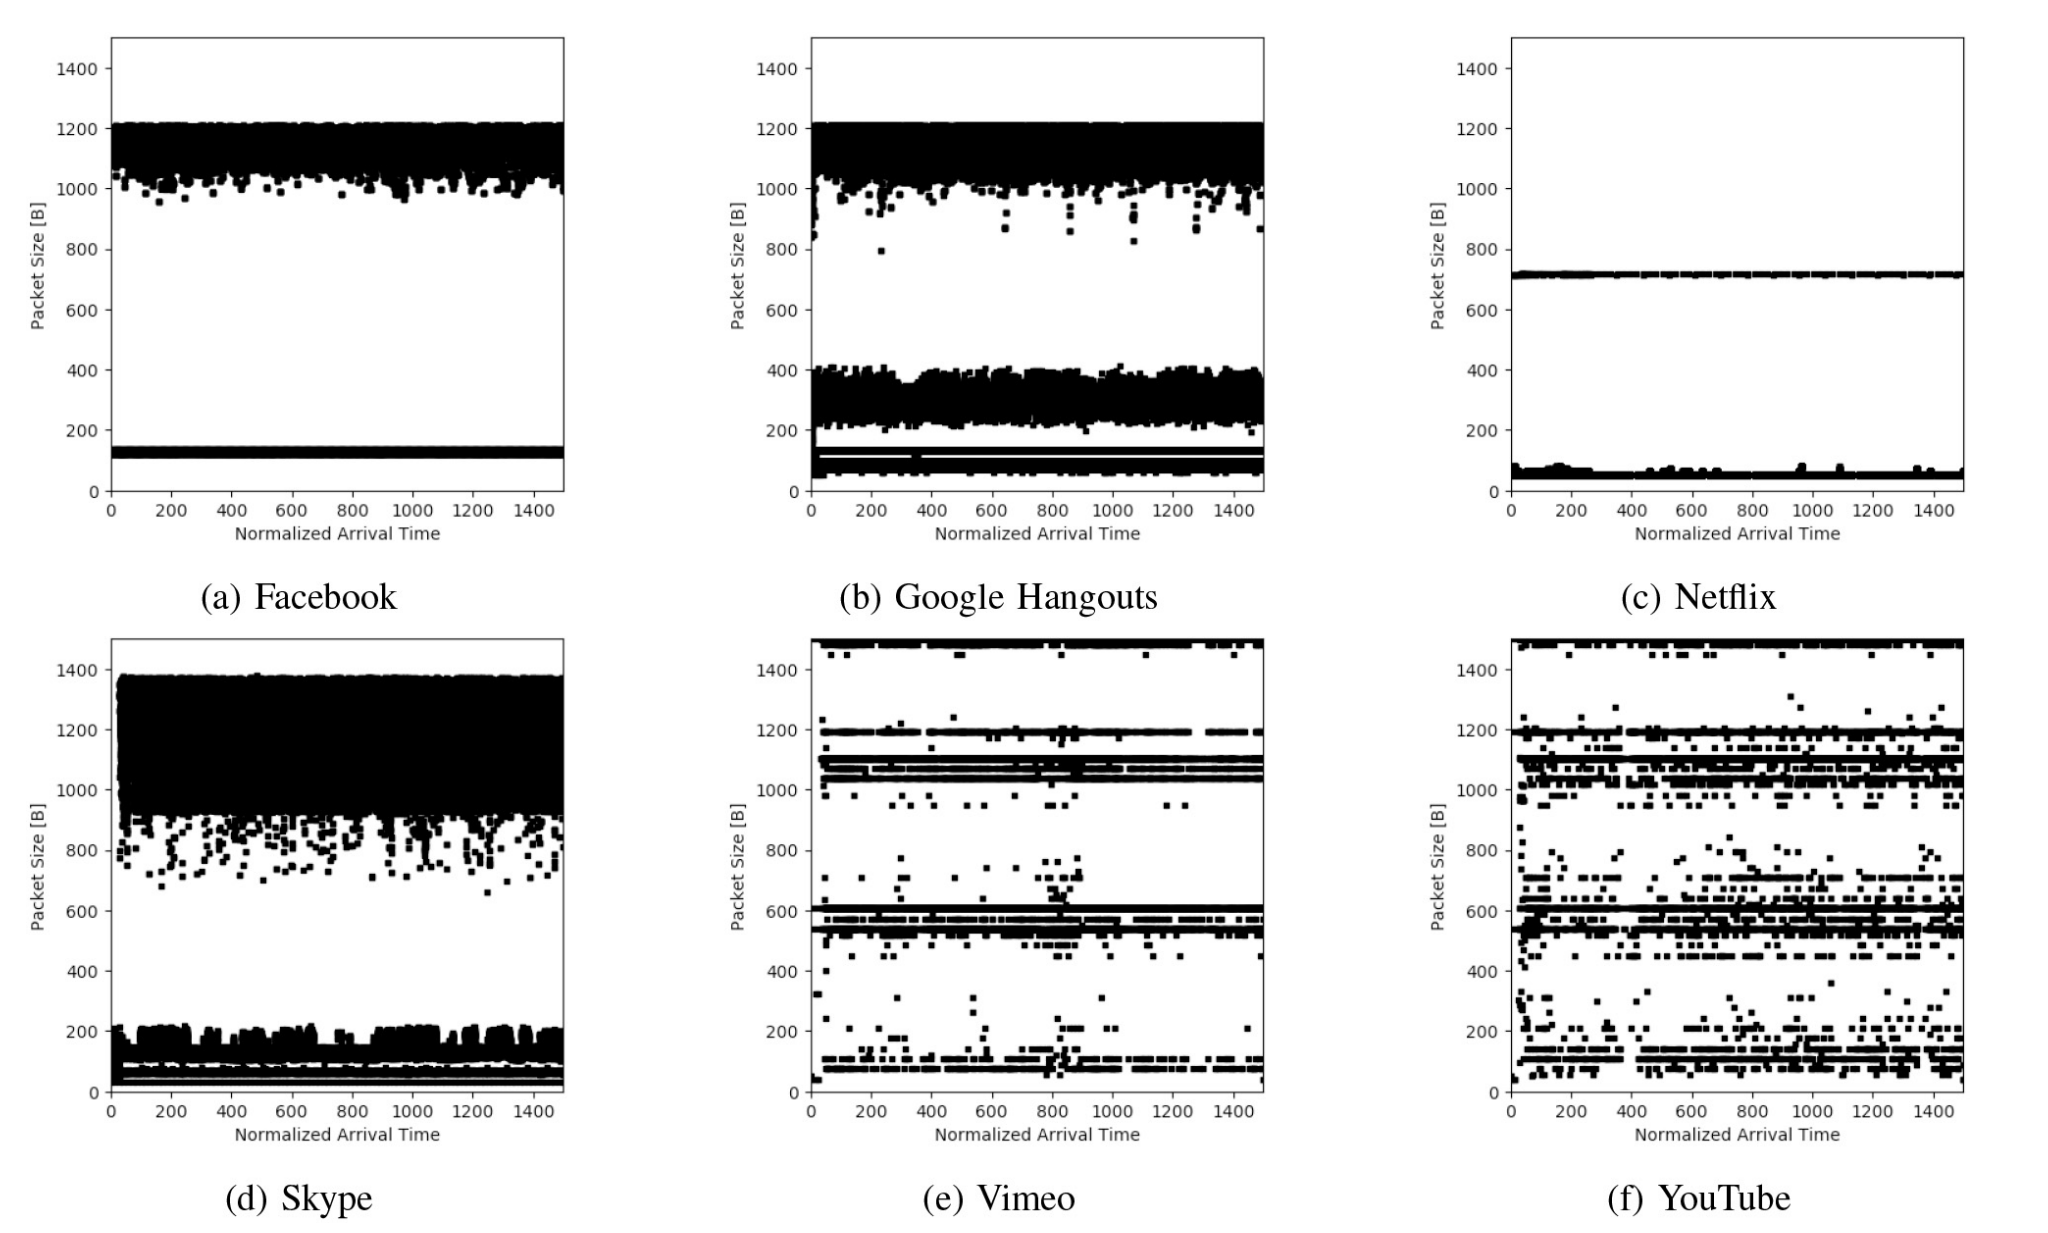
\includegraphics[width=1\textwidth]{obrazky-figures/flowpic.png}
	\caption{Příklady FlowPics pro několik video aplikací (pro ilustrační účely představují černé pixely libovolnou hodnotu v~rozmezí 1 až 255, bílé pixely představují hodnotu 0)~\cite{FlowPic}.}
	\label{flowpic}
\end{figure}

\subsection{Mini FlowPics}
\label{mini_flowpics}
Jak je uvedeno výše v~sekci~\ref{flowpic_text}, původní FlowPic obrázky mají rozlišení 1\,500$\times$1\,500 pixelů. Hodnota 1\,500 na ose $Y$ je odůvodněna schopností reprezentovat velikost každého paketu mezi 1 a~hodnotou MTU, zatímco hodnota 1\,500 na ose $X$ umožňuje vytvoření jednoduchého čtvercového obrázku.

Mini FlowPic využívají stejný konstrukční princip jako FlowPic, ale používají výrazně menší obrázky. Rozměr na ose $Y$ je zmenšen generováním histogramů, které počítají počet paketů v~určitých rozsazích délek. Rozměr na ose $X$ je zmenšen rozdělením časového intervalu na menší počet časových slotů. Mini FlowPics jsou levnější na konstrukci, trénování a~predikci, což představuje významnou výhodu~\cite{FlowPic_classification}.

Práce od Shapira \textit{et al.}~\cite{FlowPic} testovala časové bloky o~délce 120, 60, 30 a~15 sekund a~zjistila, že se rozdíl v~průměrné přesnosti zvedl o~1,25\,\%.


%=====================================================================================%
%=====================================================================================%
\chapter{Neuronové sítě}
Neuronové sítě jsou komplexní a~adaptivní statistické modely, které se inspirovaly strukturou lidského mozku. Jsou součástí širšího rámce umělé inteligence a~strojového učení, přičemž jejich hlavní charakteristikou je schopnost učit se a~adaptovat na základě zkušeností. Tento proces učení se podobá způsobu, jakým mozek zpracovává informace a~vyvozuje závěry na základě vjemů a~předchozích zkušeností~\cite{NNs}. Neuronových sítí je zároveň více druhů, v~této práci bude využívána dopředná neuronová síť, neboli \textit{feedforward neural network} (FFNN) a~také konvoluční neuronová síť (CNN).

%=====================================================================================%
\section{Různé typy neuronových sítí}
Neuronové sítě lze rozdělit do několika typů, z~nichž každá je vhodná pro různé úkoly. Mezi základní patří dopředné neuronové sítě (FFNN), které tvoří nejjednodušší architekturu a~slouží jako výchozí model pro řadu klasifikačních a~regresních úloh, konvoluční neuronové sítě (CNN), které se uplatňují zejména při analýze obrazových dat a~rekurentní neuronové sítě, neboli \textit{reccurent neural networks} (RNN), které jsou vhodné pro práci s~časovými řadami nebo sekvenčními daty.

\subsection{Dopředné neuronové sítě}
Dopředné neuronové sítě, někdy označovány jako vícevrstvé perceptrony, neboli \textit{Multilayer perceptrons} (MLP), jsou klíčovými modely hlubokého učení. Tyto modely se nazývají dopředné, protože informace proudí skrze funkci, která je vyhodnocována od vstupu $x$, přes mezi-výpočty potřebné k~definici funkce $f$, až po výstup $y$. Neexistují zde žádné zpětné vazby, kdy by výstupy modelu byly zpětně vráceny do něho samotného. Tento typ sítě má typicky tři druhy vrstev, a~to první vrstvu, která se označuje jako vstupní, pak jednu nebo více skrytých vrstev, a~poslední vrstvu, která se označuje jako výstupní. Tyto sítě mají zásadní význam pro odborníky na strojové učení. Tvoří základ mnoha důležitých komerčních aplikací, například konvoluční sítě používané pro rozpoznávání objektů na fotografiích jsou specializovaným druhem dopředných sítí, jsou také konceptuálním krokem na cestě k~rekurentním sítím, které pohánějí mnoho aplikací z~oblasti zpracování přirozeného jazyka~\cite{Goodfellow-et-al-2016}.
\begin{figure}[H]
	\centering
	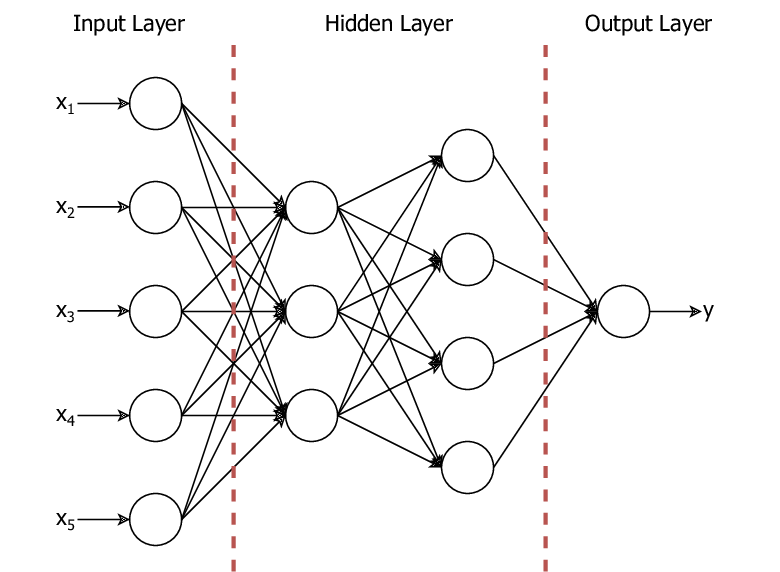
\includegraphics[width=0.6\textwidth]{obrazky-figures/ffnn.png}
	\caption{Základní architektura dopředných neuronových sítí~\cite{Schmitt2022}.}
	\label{ffnn_pic}
\end{figure}

\subsection{Konvoluční neuronové sítě}
\label{CNNs}
Konvoluční neuronové sítě jsou specializovaný typ neuronových sítí určený pro zpracování dat, která mají známou mřížkovou topologii. Příklady zahrnují časové řady, které lze považovat za jednorozměrnou mřížku odebírající vzorky v~pravidelných časových intervalech, a~obrazová data, která lze považovat za dvourozměrnou mřížku pixelů. Konvoluční sítě dosáhly obrovského úspěchu v~praktických aplikacích. Její název naznačuje, že síť používá matematickou operaci nazvanou konvoluce. Konvoluční sítě jsou jednoduše neuronové sítě, které používají konvoluci místo obvyklého maticového násobení v~alespoň jedné ze svých vrstev~\cite{Goodfellow-et-al-2016}.
\begin{figure}[hbt]
	\centering
	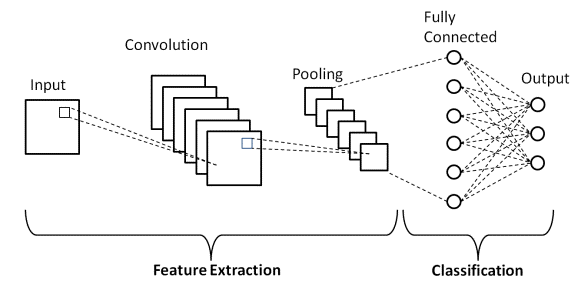
\includegraphics[width=0.7\textwidth]{obrazky-figures/cnn.png}
	\caption{Základní architektura konvolučních neuronových sítí~\cite{cnn_arch}.}
	\label{cnn_pic}
\end{figure}

\subsection{Rekurentní neuronové sítě}
Rekurentní neuronové sítě jsou rodinou neuronových sítí určených pro zpracování sekvenčních dat $x^{(1)},\dots,x^{\tau}$. Rekurentní sítě dokážou efektivně zpracovávat mnohem delší sekvence, než by bylo možné u~sítí, které na to nejsou specializovány. Většina rekurentních sítí dokáže zpracovávat sekvence proměnlivé délky. Sdílení parametrů umožňuje rozšířit a~aplikovat model na příklady různého typu (v tomto případě různé délky sekvencí) a~zobecnit je. Kdybychom měli samostatné parametry pro každou hodnotu časového indexu, nemohli bychom generalizovat na sekvence, jejichž délka nebyla během trénování viděna, ani sdílet statistickou sílu napříč různými délkami sekvencí a~pozicemi v~čase. Takové sdílení je obzvláště důležité, když se může konkrétní informace objevit na více pozicích v~rámci sekvence~\cite{Goodfellow-et-al-2016}.

%=====================================================================================%
\section{Struktura a~fungování neuronových sítí}
Neuronová síť se skládá ze vstupní vrstvy, kde se přijímají vstupy problému, skrytých vrstev, kde se určuje vztah mezi vstupy a~výstupy, a~kde jsou reprezentovány synaptickými váhami, a~výstupní vrstvy, která vysílá výstupy problému. Jednotlivé vrstvy se skládají z~několika uzlů, kterým se říká neurony, jež jsou mezi jednotlivými vrstvami propojené váženými spoji. Výstup každého uzlu závisí pouze na informacích, které jsou v~uzlu lokálně k~dispozici, ať už jsou uloženy interně, nebo přicházejí prostřednictvím vážených spojení. Každá jednotka přijímá vstupy z~mnoha jiných uzlů předává svůj výstup dalším uzlům~\cite{intro_to_nn}. Na konci je spočítána chyba (tzv. \textit{loss} funkce), které je definována jako rozdíl mezi požadovaným výstupem a~výstupem systému. Tato informace o~chybě se vrací zpět do systému a~systematicky upravuje parametry. Tento proces se opakuje, dokud není výkonnost přijatelná.

\subsection{Základní pojmy}
\label{zakladni_pojmy}
Neuronové sítě představují komplexní systémy, které se skládají z~několika klíčových komponent. Pro usnadnění orientace v~této práci je nezbytné definovat základní pojmy, které se v~souvislosti s~neuronovými sítěmi často používají.

\subsubsection*{Neuron}
Základní stavební jednotka neuronové sítě, inspirovaná biologickými neurony. Ve své podstatě je neuron optimalizován tak, aby přijímal informace od jiných neuronů, zpracovával je jedinečným způsobem a~posílal jejich výsledek dalším buňkám. Stejně jako u~biologických neuronů, umělý neuron přijímá určitý počet vstupů $x_{1}, x_{2},\dots,x_{n}$, z~nichž každý je vynásoben určitou váhou $w_{1}, w_{2},\dots,w_{n}$. Tyto vážené vstupy se sečtou dohromady, aby vznikl \textit{logit} neuronu $z=\sum_{i=0}^n w_{i}x_{i}$. Ve většině případech je součástí \textit{logitu} také \textit{bias}~\cite{dl_fundamentals}.

\subsubsection*{Vrstva}
Neurony v~lidském mozku jsou uspořádány do vrstev. Informace proudí z~jedné vrstvy do druhé, dokud se smyslový vjem nepromění v~pojmové porozumění. Podobně vzniká neuronová síť, a~to když začneme propojovat neurony mezi sebou v~různých vrstvách. První vrstva je označována jako vstrupní a~její úkol je načíst vstupní data. Poslední vrstva neuronů (výstupní vrstva) vypočítává konečnou odpověď. Prostřední vrstva (vrstvy) neuronů se nazývají skryté vrstvy, přičemž $w^{(k)}$ je váha spojení mezi neuronem ve vrstvě $k$ s~neuronem ve vrstvě $k+1$. Neurony ve stejné vrstvě mezi sebou nejsou propojeny. Skryté vrstvy mají často méně neuronů než vstupní vrstva, aby se síť naučila komprimovanou reprezentaci původního vstupu, který je zároveň i~s~výstupy vektorizovanou reprezentací~\cite{dl_fundamentals}.

\subsubsection*{Váha}
Váhy jsou parametry modelu a~určují sílu spojení mezi neurony. Každá váha $w$ řídí, jak velký vliv má jeden neuron na další. Během trénování jsou tyto váhy upravovány tak, aby minimalizovaly chybu mezi výstupem sítě a~požadovaným výstupem~\cite{Goodfellow-et-al-2016}. 

\subsubsection*{Bias}
Bias (někdy označován také jako posun) lze chápat jako klíčový parametr, který ve spojení s~váhami ovlivňuje výstup každého uzlu~\cite{NN_DL}. Bias umožňuje neuronům posunout aktivaci výstupu, což znamená, že neuron může aktivovat (nebo neaktivovat) svůj výstup i~tehdy, když jsou všechny vstupy nulové nebo když mají určité hodnoty, které by jinak vedly k~neaktivnímu stavu. Podobně jako váha je také bias při trénování upravován, aby se minimalizovala celková chyba mezi výstupem sítě a~požadovaným výstupem.

\subsubsection*{Aktivační funkce}
Aktivační funkce jsou klíčovým prvkem, který umožňuje neuronům vykazovat nelineární chování, což je zásadní pro schopnost neuronových sítí modelovat složité vzory a~vztahy mezi daty. Jsou tři základní typy, které se v~praxi využívají. Podle typu aktivační funkce lze pojmenovávat i~samotné neurony. První z~nich je \textit{sigmoid neuron}, který používá funkci: 
$$f(z) = \frac{1}{1+e^{-z}}.$$
V praxi to znamená, že když je logit velmi malý, výstup neuronu je velmi blízko 0, a~když je velmi velký, výstup je blízko 1~\cite{dl_fundamentals}.

Dalším z~používaných je \textit{tanh neuron}, který využívá podobný druh nelinearity jako \textit{sigmoid neuron}, ale namísto rozsahu 0 až 1 se výstup \textit{tanh neuronů} pohybuje v~rozmezí -1 až 1~\cite{dl_fundamentals}. Funkce, kterou neuron používá je, jak již název napovídá, následující: 
$$f(z) = \tanh{(z)}.$$

Poslední typ, který poslední dobou získává více a~více popularity a~je hojně využívaný, je \textit{restricted linear unit (ReLU) neuron}, který závádí odlišný typ nelinearity než předchozí dvě aktivační funkce~\cite{dl_fundamentals}. V~praxi to znamená, že když je logit záporný, výstup je nulový, a~když je logit kladný, jeho hodnota se nemění. Matematicky lze funkci vyjádřit následovně:
$$f(z) = \max\,(0,z).$$

%=====================================================================================%
\section{Trénování neuronových sítí}
Trénink modelu znamená iterativní úpravu jeho parametrů, jako jsou váhy a~biasy, s~cílem minimalizovat rozdíl mezi výstupy modelu a~očekávanými výsledky. Tento rozdíl je měřen pomocí ztrátové funkce, která kvantifikuje výkon modelu a~slouží k~optimalizaci. Fáze trénování zahrnuje dva hlavní kroky: dopředný a~zpětný průchod sítí. Nejprve jsou vstupní data poslána dopředu, kde model na základě svých aktuálních parametrů vytvoří předpovědi. Následně se spočítá chyba mezi těmito předpověďmi a~skutečnými výstupy. Tato chyba se následně využije ve zpětném průchodu, kde se pomocí výpočtu gradientů ztrátové funkce aktualizují parametry modelu. Tento proces se opakuje v~mnoha iteracích, dokud model nenajde optimální hodnoty parametrů, které minimalizují chybu a~zajišťují co nejlepší výkon~\cite{dl_fundamentals}. Jedním z~nejvíce používaných algoritmus je zpětné propagace, neboli \textit{backpropagation}.

\subsection{Backpropagation}
Pokud používáme neuronovou síť typu feedforward, která přijímá vstup $x$ a~generuje výstup $\hat{y}$, informace procházejí sítí směrem vpřed. Vstup $x$ poskytuje počáteční data, která se postupně šíří skrz skryté jednotky v~jednotlivých vrstvách a~nakonec vedou k~výstupu $\hat{y}$. Tento proces je známý jako dopředná propagace, neboli \textit{forward propagation}~\cite{Goodfellow-et-al-2016}.

Během trénování může dopředná propagace pokračovat, dokud nevytvoří skalární hodnotu ztrátové funkce $J(\theta)$. Algoritmus zpětné propagace, často jednoduše nazývaný \textit{back\-prop}, umožňuje, aby informace o~ztrátě následně proudily zpětně sítí, aby bylo možné vypočítat ~\cite{Goodfellow-et-al-2016}.

% optimalizacni algoritmus
Termín zpětná propagace je často mylně chápán jako celý učící algoritmus pro vícevrstvé neuronové sítě. Ve skutečnosti zpětná propagace označuje pouze metodu pro výpočet gradientu, zatímco jiný algoritmus, například stochastický gradientní sestup, je použit k~provádění učení na základě tohoto gradientu. Dále je zpětná propagace často mylně považována za specifickou pro vícevrstvé neuronové sítě, ale v~principu může vypočítat derivace jakékoliv funkce (u některých funkcí je správnou odpovědí, že derivace funkce je nedefinovaná)~\cite{Goodfellow-et-al-2016}.

%=====================================================================================%
\section{Supervised learning}
Učení s~učitelem, neboli \textit{supervised learning}, představuje velkou část výzkumné činnosti v~oblasti strojového učení. Definující charakteristikou učení s~učitelem je dostupnost anotovaných trénovacích dat, na rozdíl od učení bez dohledu, neboli \textit{unsupervised learning}, kdy algoritmus musí odvodit vzory a~struktury pouze z~neoznačených dat. Název naznačuje představu „učitele“, který instruuje učící se systém, jaké štítky přiřadit k~trénovacím příkladům. Tyto štítky jsou obvykle třídy v~úlohách klasifikace. Učení spočívá v~naučení se mapování mezi sadou vstupních proměnných $X$ a~výstupní proměnnou $Y$ a~následném použití tohoto mapování k~predikci výstupů pro dosud neviděná data~\cite{Cunningham2008}. 

Tradiční přístupy učení s~učitelem jsou silně závislé na množství dostupných anotovaných trénovacích dat. I~když je k~dispozici obrovské množství dat, nedostatek anotací vedl výzkumníky k~hledání alternativních přístupů, které je dokážou využít. V~tomto kontextu hrají \textit{self-supervised} metody klíčovou roli v~podpoře pokroku hlubokého učení bez nutnosti nákladných anotací~\cite{technologies9010002}.

\subsection{Self-supervised learning}
\textit{Self-supervised learning} (SSL) představuje způsob, jak využít neoznačená data k~učení základních reprezentací, čímž se eliminuje závislost na ručně anotovaných trénovacích datech. Místo explicitních anotací si model generuje vlastní pseudoznačky, což umožňuje učení přímo z~dat bez nutnosti lidského zásahu.

V poslední době se v~metodách SSL kombinují jak generativní, tak kontrastivní přístupy. Generativní metody se zaměřují na modelování dat tak, aby model mohl generovat nebo rekonstruovat jejich části, zatímco kontrastivní metody se soustředí na učení reprezentací tím, že rozlišují mezi podobnými a~odlišnými vzory. Mezi oblíbené techniky patří navrhování různých pretextových úloh, které pomáhají modelům učit se reprezentace dat pomocí pseudoznaček. Příklady těchto pretextových úloh zahrnují malování obrázků, kolorování černobílých obrázků, skládání obrázků z~rozbitých částí (tzv. \textit{jigsaw puzzles}), superrozlišení, predikci následujících snímků ve videu nebo audiovizuální korespondence. Tyto úlohy se ukázaly jako efektivní pro učení silných reprezentací, které lze následně využít pro širokou škálu \textit{downstream} úkolů, jako je klasifikace nebo detekce objektů~\cite{technologies9010002}.

\subsection{Kontrastivní učení}
\label{contrastive_learning}
Kontrastivní učení, neboli \textit{contrastive learning} (CL), je diskriminační přístup, který se zaměřuje na seskupování podobných vzorků blíže k~sobě a~odlišných vzorků dál od sebe, jak je znázorněno na obrázku~\ref{cl}. k~dosažení tohoto cíle se používá metrika podobnosti, která měří, jak blízko jsou dva embeddingy, neboli číselné reprezentace dat ve vektorovém prostoru. Zejména pro úkoly počítačového vidění se hodnotí kontrastní ztráta na základě reprezentací vlastností obrázků, které jsou získány z~enkodéru. Například je vybrán jeden vzorek z~trénovacího datasetu a~jeho transformovaná verze je získána aplikací vhodných technik augmentace dat. Během trénování je augmentovaná verze původního vzorku považována za pozitivní vzorek, a~zbytek vzorků v~dávce (tzv. \textit{batch)}/datasetu (záleží na použité metodě) je považován za negativní vzorky. Model je následně trénován tak, aby se naučil odlišovat pozitivní vzorky od negativních~\cite{technologies9010002}.
\begin{figure}[hbt]
	\centering
	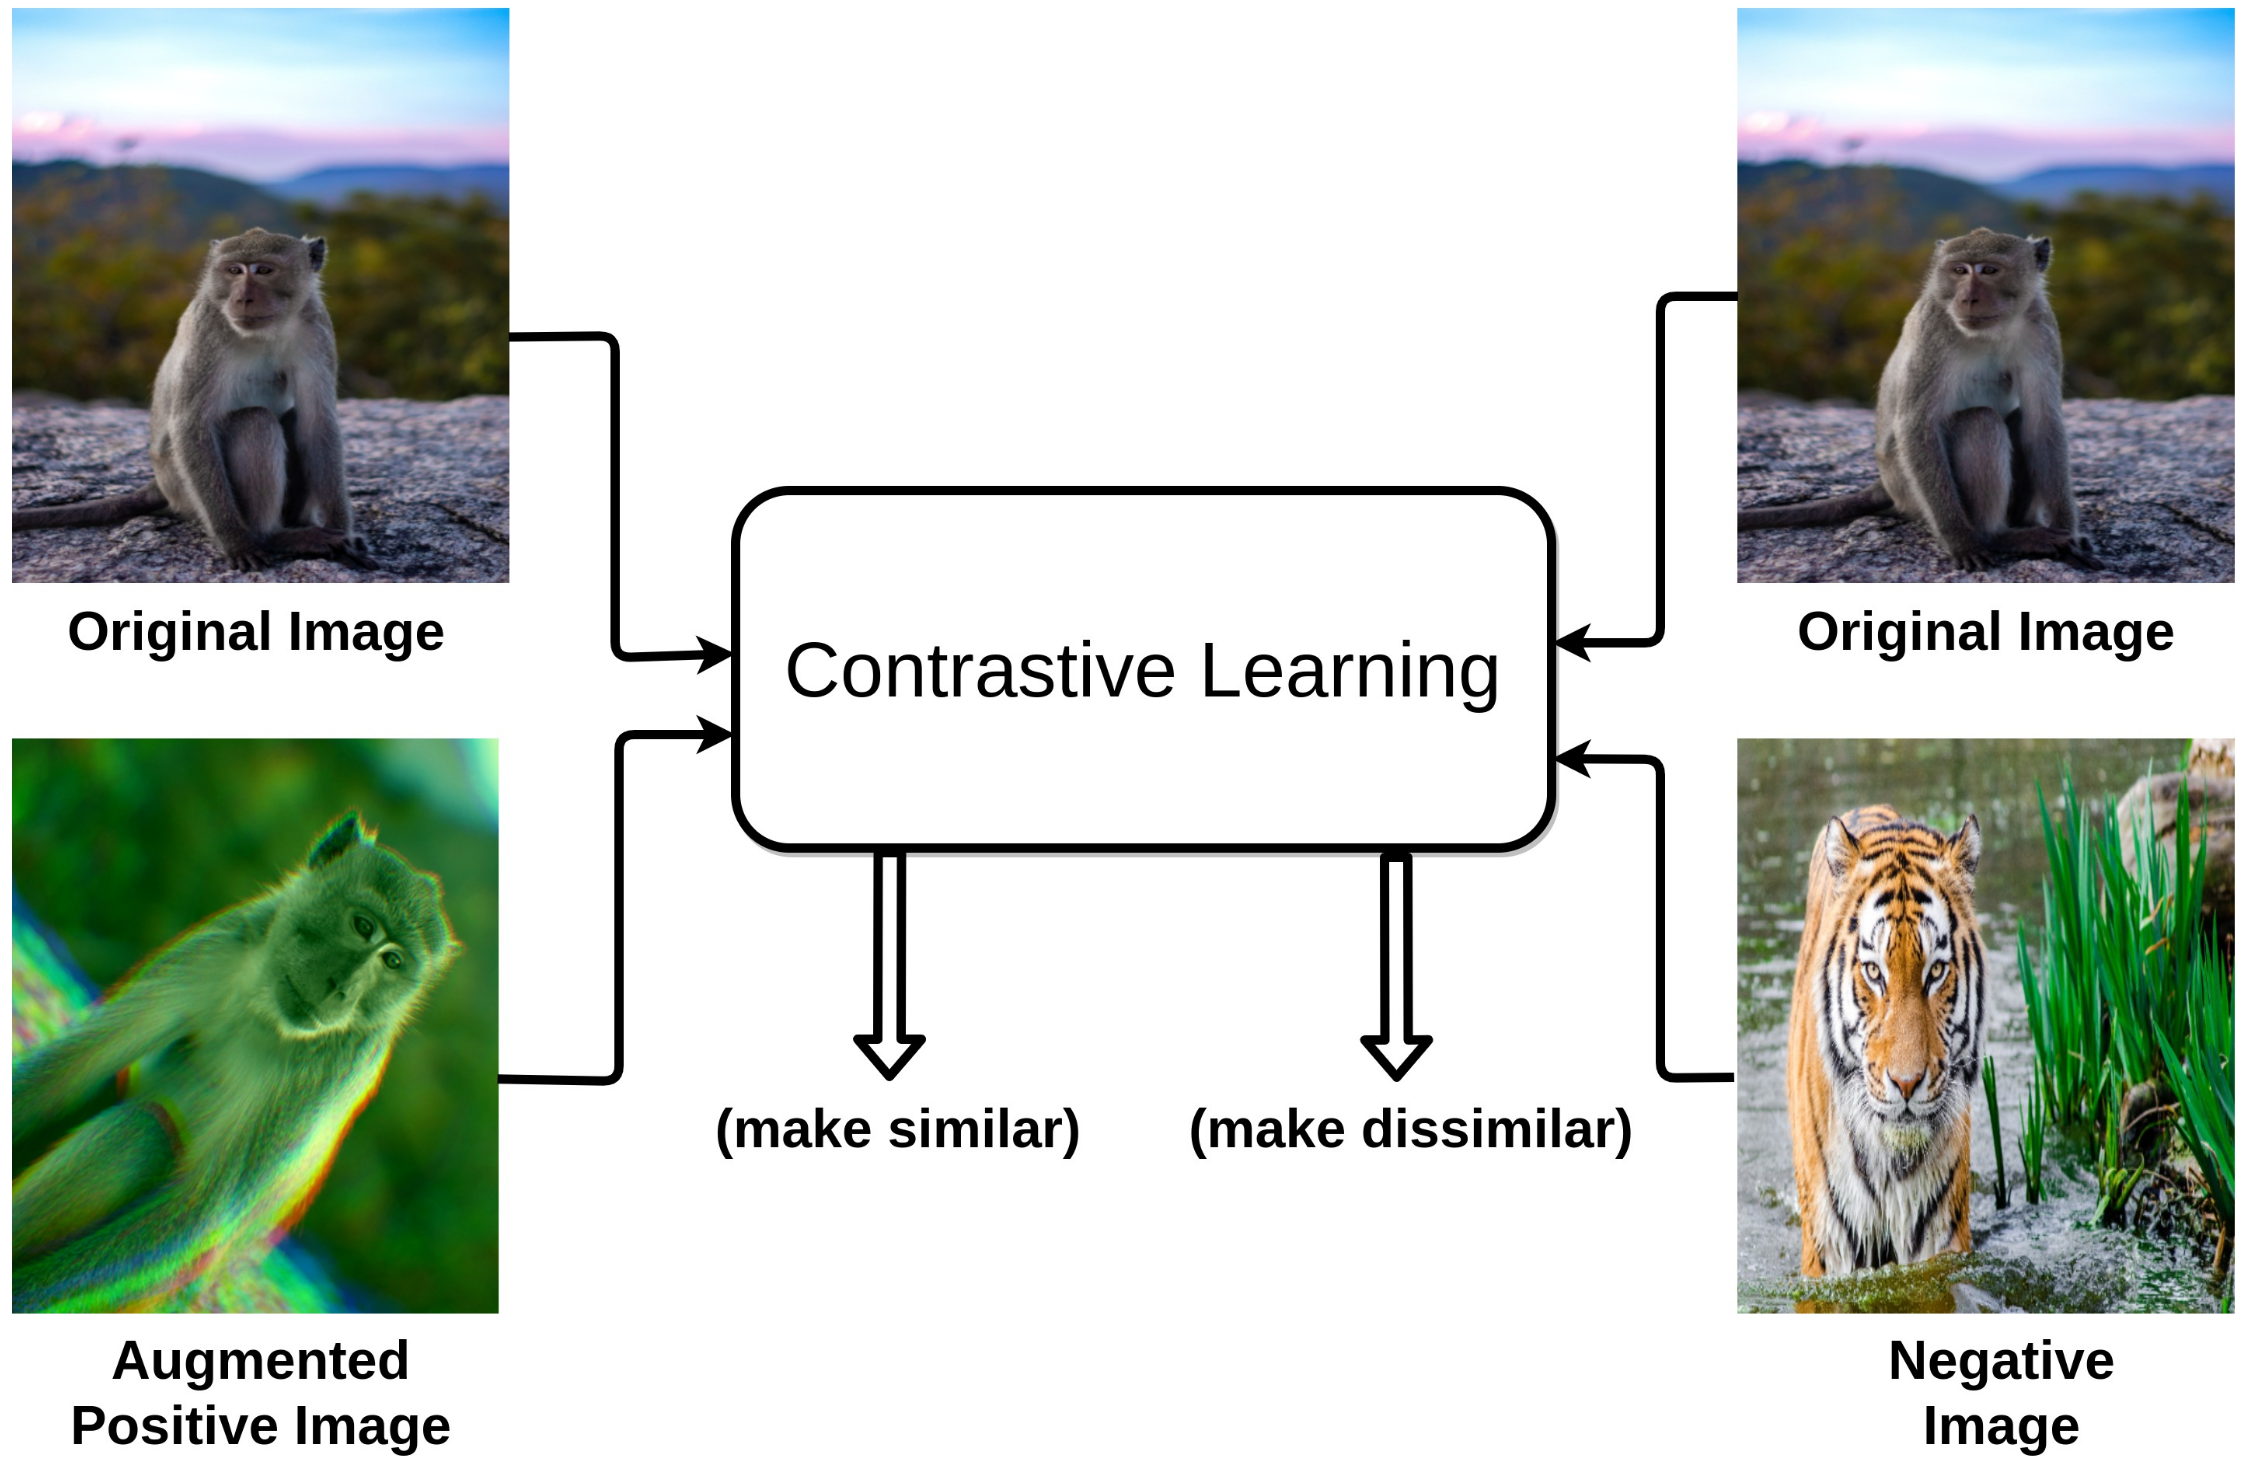
\includegraphics[width=0.6\textwidth]{obrazky-figures/cl.png}
	\caption{Základní intuice paradigmatu kontrastního učení, přiblížit původní a~augmentované obrázky a~oddálit původní a~negativní~\cite{technologies9010002}.}
	\label{cl}
\end{figure} 

\subsection{SimCLR}
\label{simclr_text}
\textit{SimCLR} je framework pro kontrastivní učení vizuálních reprezentací. \textit{SimCLR} se učí reprezentace 
maximalizováním shody mezi různě augmentovanými pohledy na stejný datový vzorek pomocí kontrastní ztráty v~latentním prostoru. 
Metoda náhodně vybere $N$ vzorků (tzv. \textit{minibatch}) a~definuje kontrastní predikční úlohu pro páry augmentovaných vzorků, 
které jsou z~této skupiny vzorků odvozeny, což vede k~$2N$ datovým bodům. Negativní vzorky nejsou explicitně vybírány. Místo toho, 
pokud je dán pozitivní pár, ostatní $2(N - 1)$ augmentované vzorky ve zmíněné skupině vzorků (\textit{minibatch}) jsou považovány za negativní vzorky~\cite{simclr}.

\begin{figure}[H]
	\centering
	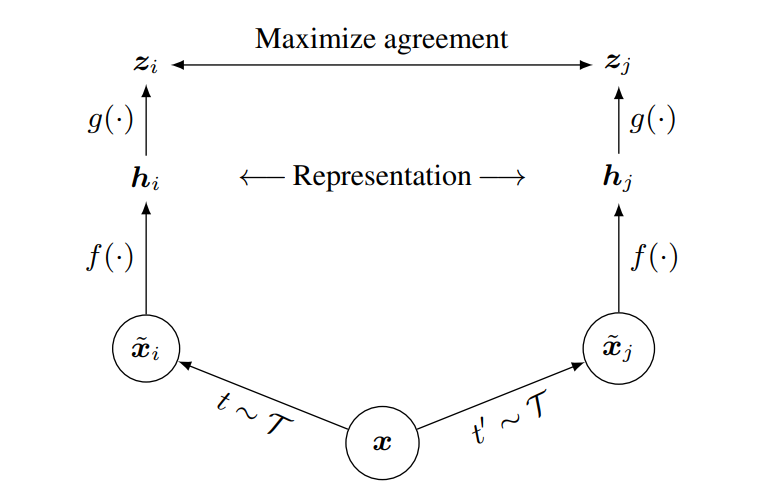
\includegraphics[width=0.6\textwidth]{obrazky-figures/simclr.png}
	\caption{Ilustrace tréninkového procesu pomocí metody SimCLR, kde $x$ je vstupní vzorek, $\mathcal{T}$ je rodina validních augmentací, $t$ je vybraná transformace, $\tilde{x}_i$ a~$\tilde{x}_j$ jsou augmentované pohledy, $f(\cdot)$ je základní neuronová síť (\textit{encoder}), $h_i$ a~$h_j$ jsou reprezentace z~augmentovaných vzorků, $g(\cdot)$ je projekční hlava, která mapuje reprezentace do latentního prostoru a~$z_i$, $z_j$ jsou latentní reprezentace~\cite{simclr}.}
	\label{simclr}
\end{figure}

\subsection{Ztrátová funkce}
\label{loss_func}
Ztrátová funkce, neboli \textit{loss function} (také označována jako \textit{cost function}), je funkce, která měří rozdíl mezi výstupem sítě a~očekávaným výsledkem. Ztrátová funkce slouží jako optimalizační kritérium během trénování modelu, přičemž usměrňuje úpravy jeho parametrů s~cílem minimalizovat chybu. Volba vhodné ztrátové funkce hraje zásadní roli, jelikož výrazně ovlivňuje schopnost modelu efektivně se učit a~zobecňovat získané poznatky~\cite{NN_DL}.

Ztrátová funkce využívaná metodou \textit{SimCLR}, která je definována v~sekci~\ref{simclr_text}, je označována jako \textit{NT-Xent} (\textit{Normalized Temperature-scaled Cross Entropy Loss}) a~definována následovně~\cite{simclr}:
$$\ell_{i,j} = -\log \frac{\exp(\text{sim}(z_i, z_j) / \tau)}{\sum_{k=1}^{2N} \mathds{1}_{[k \neq i]} \exp(\text{sim}(z_i, z_k) / \tau)},$$
kde:
\begin{itemize}
    \item sim($z_{i}, z_{k}$) je kosinová podobnost mezi reprezentacemi $z_{i} \text{ a~} z_{j}$,
    \item $\tau$ je teplotní parametr,
    \item $\mathds{1}_{[k \neq i]} \in \{0,1\}$ je indikátor, že funkce vyhodnocuje 1, pokud $k \neq i$.
\end{itemize}

%=====================================================================================%
\section{Augmentace dat}
\label{augmentace}
Jednou z~možností, jak zlepšit generalizaci modelu a~eliminovat přeučení (\textit{overfitting}), je trénovat ho na větším množství dat. V~praxi ho však máme jen omezené množství. U~některých úloh strojového učení je celkem snadné vytvořit nová, umělá data. Tento přístup je nejjednodušší u~klasifikace. Klasifikátor musí vzít složitý, vysoce dimenzionální vstup $x$ a~shrnout ho do jediné kategorie $y$. To znamená, že hlavním úkolem klasifikátoru je být invariantní vůči široké škále transformací. Nové páry $(x, y)$ můžeme snadno generovat jednoduše tím, že transformujeme vstupy $x$ v~trénovacím datasetu~\cite{Goodfellow-et-al-2016}.

Jelikož se tato práce zabývá klasifikací síťového provozu, augmentace relevantní pro tuto práci se týkají modifikace síťových toků. Ty lze augmentovat několika způsoby, mezi které patří časový posun v~paketech (\textit{inter-arrival time}, IAT), změna obousměrného zpoždění (označováno jako \textit{round-trip time}, RTT), změna směru toku a~v~neposlední řadě vynechání paketů v~toku~\cite{flowpic_augmentations}.

V~metodě SimCLR, využívané v~této práci, jsou augmentace dat klíčovou součástí procesu. Pomocí vybraných augmentací budou vytvářeny pozitivní páry, které jsou důležité pro ztrátovou funkci popsanou v~sekci~\ref{loss_func}.

\subsection{Modifikace RTT}
Obousměrné zpoždění (RTT) v~internetových sítích se pohybuje v~rozmezí od několika milisekund až po malé zlomky sekundy. Vzhledem k~mechanismům řízení přetížení v~protokolu TCP a~řízení toku na aplikační vrstvě se změny v~RTT téměř lineárně promítají do rozložení paketů podél časové osy. Kromě těchto faktorů může změna RTT nastat také v~důsledku dalších situací, častými příčinami změn jsou také přetížení síťových zařízení a~ztráta paketů~\cite{flowpic_augmentations}. 

Pro simulaci změny RTT násobíme čas příchodu každého paketu faktorem $\alpha$. Faktor $\alpha$ je vybírán rovnoměrně v~intervalu [$\alpha_{min}, \alpha_{max}$], tedy $RTT_{new} = \alpha * RTT_{old}$~\cite{flowpic_augmentations}.

\begin{figure}[H]
	\centering
	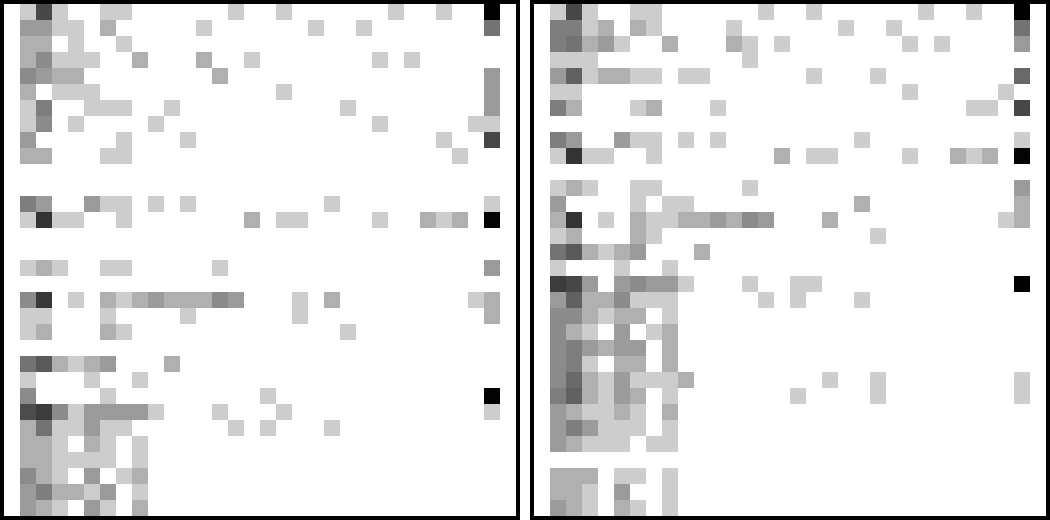
\includegraphics[width=0.6\textwidth]{obrazky-figures/rtt_and_orig.png}
	\caption{Rozdíl mezi originální FlowPic reprezentací (vlevo) a~augmentovanou verzí (vpravo).}
	\label{flowpic_rtt}
\end{figure}


\subsection{Modifikace IAT}
Častými příčinami změny IAT jsou síťová přetížení a~nárazové zátěže. Při síťovém přetížení může být generování paketů zpomaleno, což vede k~delším časovým intervalům mezi příjmy paketů, čímž dochází k~prodloužení IAT. Naopak, v~případě nárazových zátěží, kdy síť najednou obdrží vysoký objem dat může být čas mezi příjmy paketů zkrácen~\cite{flowpic_augmentations}. 

Posun v~čase lze simulovat přidáním konstanty $b \in [b_{min}, b_{max}]$ k~času příchodu každého paketu. Konstantní hodnota $b$ je rovnoměrně vzorkována z~intervalu $U[b_{min}, b_{max}]$, což znamená, že $t_{new} = t_{old} + b$~\cite{simclr}.

\begin{figure}[H]
	\centering
	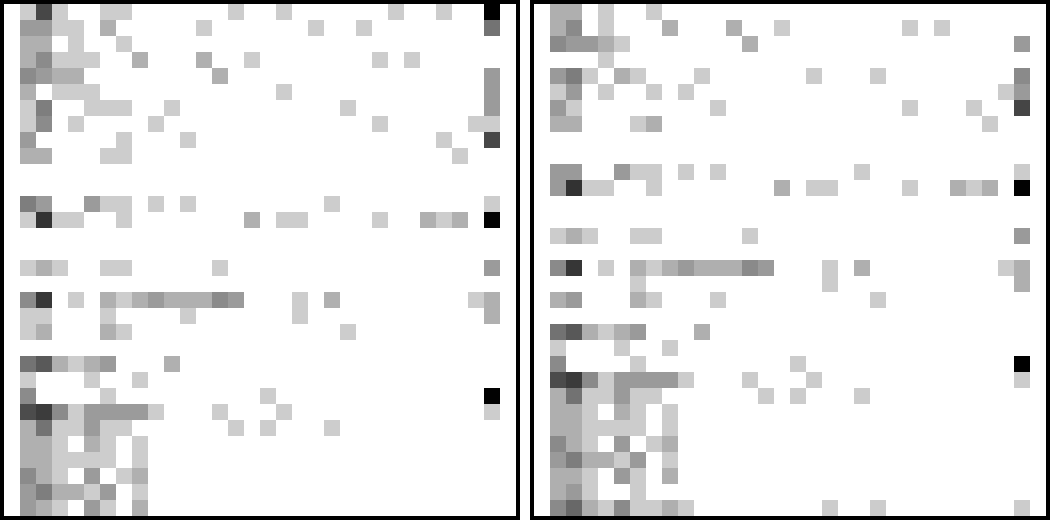
\includegraphics[width=0.6\textwidth]{obrazky-figures/iat_and_orig.png}
	\caption{Rozdíl mezi originální FlowPic reprezentací (vlevo) a~augmentovanou verzí (vpravo).}
	\label{flowpic_iat}
\end{figure}

\subsection{Vynechání paketů}
Ztráty (vynechání) paketů, jsou častým jevem v~sítích. Existuje několik metod simulace ztráty paketů, které mohou zohlednit komplexní chování, jako je přetížení síťových zařízení, špatná kvalita připojení nebo řízení přetížení v~protokolu TCP. Simulaci lze provést na jednoduchém procesu ztráty, při němž jsou všechny pakety odstraněny v~časovém intervalu $[t \-- \Delta t, t + \Delta t]$. Hodnota $t$ je náhodně vybrána v~rámci časového intervalu relace a~$\Delta t$ představuje délku tohoto intervalu~\cite{flowpic_augmentations}.

\begin{figure}[H]
	\centering
	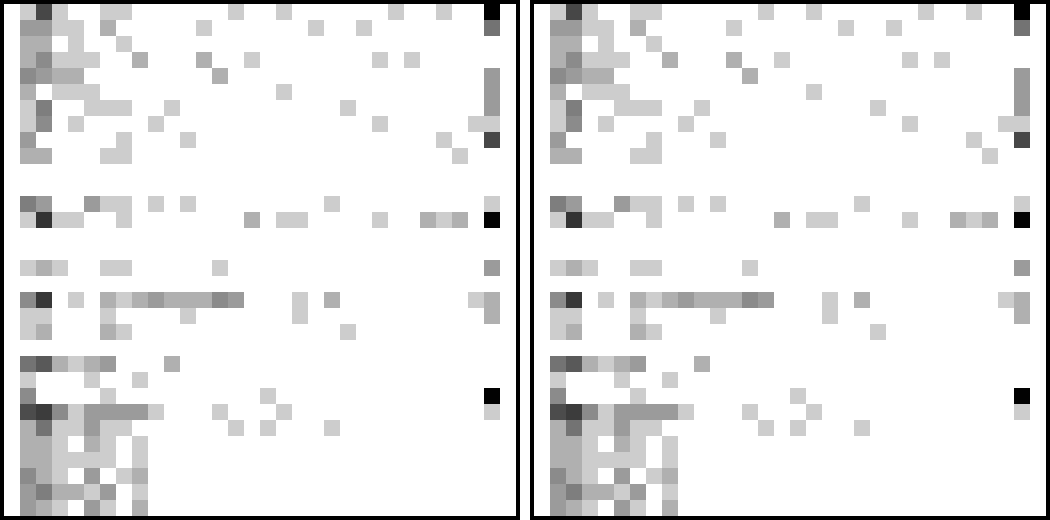
\includegraphics[width=0.6\textwidth]{obrazky-figures/pktl_and_orig.png}
	\caption{Rozdíl mezi originální FlowPic reprezentací (vlevo) a~augmentovanou verzí (vpravo).}
	\label{flowpic_pktl}
\end{figure}

Na první pohled vypadají obě reprezentace velmi podobně. Vzhledem k~náhodné délce vynechaného intervalu může být rozdíl mezi nimi minimální. Tato změna se ve FlowPic reprezentaci projeví pouze drobnou odchylkou v~intenzitě některých pixelů, což nemusí být vizuálně patrné.

\subsection{FlowPic augmentace}
\label{flowpic_augmentace}
V oblasti počítačového vidění existuje široká škála známých transformací obrazů, mezi které patří například převrácení, úprava barev, ořez, rotace, přidání šumu nebo náhodné vymazání částí obrazu. Při aplikaci těchto transformací na FlowPic je však třeba zohlednit, že mohou zásadně změnit významné charakteristiky obrazu. V~důsledku toho nelze jednoznačně určit užitečnost konkrétní transformace pro augmentaci pouze na základě vizuálního posouzení výsledného obrazu. Například populární transformace rotace může u~FlowPicu výrazně změnit rozložení velikosti paketů v~čase, čímž dochází k~deformaci významných rysů a~narušení informací nezbytných pro proces učení~\cite{flowpic_augmentations}. 

Některé augmentace využívané v~počítačovém vidění i~přes to použít lze, například horizontální otočení je akceptovatelné pro periodické signály jako jsou video a~VoIP, kde jsou relace dlouhé a~obraz se podél horizontální osy významně nemění. Experimentovat lze také s~malými rotacemi v~rámci několika jednotek stupňů, jak je ukázáno na porovnání~\ref{flowpic_rotation}.

Přesto se ukazuje jako efektivnější aplikovat augmentace přímo na síťový tok ještě před jeho transformací do FlowPic reprezentace, protože manipulace s~původním tokem umožňuje zachovat a~lépe reflektovat jeho klíčové vlastnosti a~statistiky~\cite{flowpic_augmentations}.
\begin{figure}[H]
	\centering
	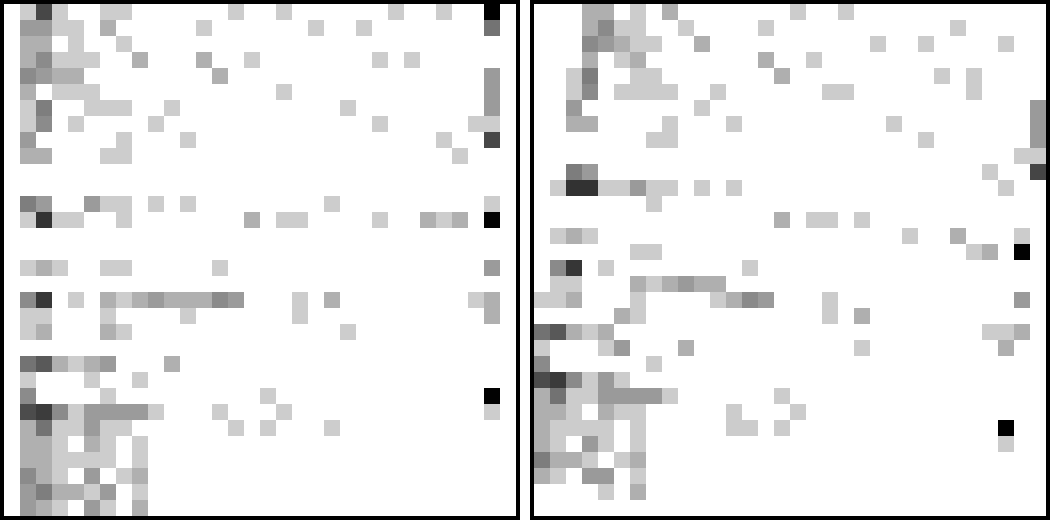
\includegraphics[width=0.6\textwidth]{obrazky-figures/rotation_and_orig.png}
	\caption{Rozdíl mezi originální FlowPic reprezentací (vlevo) a~rotovanou verzí (vpravo).}
	\label{flowpic_rotation}
\end{figure}

%=====================================================================================%
%=====================================================================================%
\chapter{Návrh řešení}
Tato kapitola popisuje datové sady, které budou využity pro trénování modelu a~následné porovnání s~výsledky dosažených v~referenční práci~\cite{flowpic_augmentations}. Zároveň je zde popsán navrhovaný model obsahující jak \textit{encoder} $f(\cdot)$, tak projekční hlavu $g(\cdot)$. Definován je zde také lineární model sloužící k~výsledné klasifikaci, který v~podstatě při tzv. \textit{fine tuningu} v~konečné fázi nahradí vícevrstvý perceptron $g(\cdot)$. Součástí návrhu řešení je také popis samotného trénování a~aplikace augmentací.


%=====================================================================================%
\section{Datové sady}
\label{datasets}
K~tomu, aby bylo možné efektivně trénovat neuronovou síť, je nezbytné mít k~dispozici dostatečně velké množství dat. Tato práce bude pracovat se čtyřmi různými datasety: Mirage19~\cite{mirage19}, Mirage22~\cite{mirage22}, Ucdavis-icdm19~\cite{usdavis} a~UTMobileNetTraffic2021~\cite{UTMobileNetTraffic}. Každý z~těchto datasetů je rozdělen na trénovací část, která obsahuje největší množství dat a~slouží k~učení modelu, validační část, která se využívá ke sledování výkonnosti modelu během trénování a~k~optimalizaci jeho hyperparametrů a~testovací část, která je určena pro finální vyhodnocení výkonu modelu na dosud neviděných datech, aby bylo možné objektivně posoudit jeho generalizaci.

\subsection{Mirage19}
\label{mirage19_sekce}
Dataset mirage19 zahrnuje síťový provoz generovaný 40 aplikacemi pro Android, které spadají do 16 různých kategorií dle klasifikace portálu pro distribuci aplikací Google Play. Celkem bylo v~rámci datasetu shromážděno 4\,606 \textit{PCAP} záznamů~\cite{mirage19}.

Společné vlastnosti, které dataset popisuje jsou ID toku, zdrojová a~cílová IP adresa, zdrojový a~cílový port, protokol, čas prvního a~posledního paketu, směr paketů, délka paketů, flagy, informace o~označení (\textit{label}), celkový počet paketů a~Android aplikace, ze které byl síťový provoz zachycen.

\begin{table}[H]
    \centering
    \resizebox{\textwidth}{!}{%
        \begin{tabular}{l c c c c c c c}
            \toprule
            \textbf{Název} & \textbf{Rozdělení} & \textbf{Filtry} & \textbf{Třídy} & \textbf{Počet toků} &  \makecell{\textbf{Průměrná délka}\\ \textbf{toku}} & \makecell{\textbf{Průměrný počet}\\ \textbf{paketů}} \\
            \midrule
            \multirow{3}{*}{Mirage19} 
              & train & \multirow{3}{*}{\centering\makecell{žádný}} & \multirow{3}{*}{20} & 51\,798 & 28,62\,s & 30,33\\
              & val   &  & & 5\,776 & 28,40\,s & 30,43\\
              & test  &  & & 6\,418 & 26,66\,s & 30,33\\
            \bottomrule
        \end{tabular}
    }
    \caption{Analýza datové sady Mirage19 bez filtru.}
    \label{mirage19_no_filter}
\end{table}

\begin{table}[H]
    \centering
    \resizebox{\textwidth}{!}{%
        \begin{tabular}{l c c c c c c c}
            \toprule
            \textbf{Název} & \textbf{Rozdělení} & \textbf{Filtry} & \textbf{Třídy} & \textbf{Počet toků} &  \makecell{\textbf{Průměrná délka}\\ \textbf{toku}} & \makecell{\textbf{Průměrný počet}\\ \textbf{paketů}} \\
            \midrule
            \multirow{3}{*}{Mirage19} 
              & train & \multirow{3}{*}{\centering\makecell{>30pkts}} & \multirow{3}{*}{20} & 38\,959 & 20,52\,s & 31,89\\
              & val   &  & & 4\,402 & 28,40\,s & 31,89\\
              & test  &  & & 4\,818 & 26,66\,s & 31,89\\
            \bottomrule
        \end{tabular}
    }
    \caption{Analýza datové sady Mirage19 s~filtrem >30pkts.}
    \label{mirage19_filter}
\end{table}

Pro datovou sadu byl zvolen filtr, který zpracovává pouze toky s~více než 30 pakety. Na rozdíl od referenčních prací~\cite{huawei_paper}, které volily filtr s~hranicí 10 paketů, byla tato vyšší hodnota zvolena z~důvodu, že použitá datová sada neobsahuje toky kratší než 10 paketů a~zároveň obsahuje pouze malé množství toků kratších 20 paketů, konkrétně pouze 1,09\,\%.

\begin{figure}[H]
	\centering
	
\includegraphics[width=0.6\textwidth]{obrazky-figures/m19_flowpics.png}
	\caption{FlowPic reprezentace vytvořené z~dvou náhodně vybraných toků z~datové sady Mirage19 bez filtru.}
	\label{m19_flowpic}
\end{figure}

\begin{figure}[H]
	\centering
	
\includegraphics[width=0.6\textwidth]{obrazky-figures/f_m19_flowpics.png}
	\caption{FlowPic reprezentace vytvořené z~dvou náhodně vybraných toků z~datové sady Mirage19 s~filtrem.}
	\label{f_m19_flowpic}
\end{figure}

Jak lze pozorovat na FlowPic reprezentacích, tato datová sada není pro vytváření FlowPiců příliš vhodná, což se projeví na finální přesnosti modelu.

\subsection{Mirage22}
Tento dataset obsahuje data zachycená z~provozu devíti mobilních aplikací, které za doby pandemie COVID-19 zaznamenaly velký růst. Ony aplikace jsou Discord, GotoMeeting, Meet, Messenger, Skype, Slack, Teams, Webex a~Zoom. Trénovací část obsahuje celkem 21\,685 vzorků, validační 2\,410 a~trénovací 2\,678. Celkový počet tříd činí 9~\cite{mirage22}.

\begin{table}[H]
    \centering
    \resizebox{\textwidth}{!}{%
        \begin{tabular}{l c c c c c c c}
            \toprule
            \textbf{Název} & \textbf{Rozdělení} & \textbf{Filtry} & \textbf{Třídy} & \textbf{Počet toků} &  \makecell{\textbf{Průměrná délka}\\ \textbf{toku}} & \makecell{\textbf{Průměrný počet}\\ \textbf{paketů}} \\
            \midrule
            \multirow{3}{*}{Mirage22} 
              & train & \multirow{3}{*}{\centering\makecell{>10pkts}} & \multirow{3}{*}{9} & 21\,685 & 333,28\,s & 6\,708,65\\
              & val   &  &  & 2\,410 & 316,36\,s & 6\,370,42\\
              & test  &  &  & 2\,678 & 309,81\,s & 7\,258,81\\
            \bottomrule
        \end{tabular}
    }
    \caption{Analýza datové sady Mirage22 s~filtrem >10pkts.}
    \label{mirage22_filter_10}
\end{table}

\begin{table}[H]
    \centering
    \resizebox{\textwidth}{!}{%
        \begin{tabular}{l c c c c c c c}
            \toprule
            \textbf{Název} & \textbf{Rozdělení} & \textbf{Filtry} & \textbf{Třídy} & \textbf{Počet toků} &  \makecell{\textbf{Průměrná délka}\\ \textbf{toku}} & \makecell{\textbf{Průměrný počet}\\ \textbf{paketů}} \\
            \midrule
            \multirow{3}{*}{Mirage22} 
              & train & \multirow{3}{*}{\centering\makecell{>1\,000pkts}} & \multirow{3}{*}{9} & 3\,700 & 614.51\,s & 39\,466,81\\
              & val   &  &  & 412 & 617,08\,s & 37\,571,55\\
              & test  &  &  & 457 & 588,74\,s & 35\,279,41\\
            \bottomrule
        \end{tabular}
    }
    \caption{Analýza datové sady Mirage22 s~filtrem >1\,000pkts.}
    \label{mirage22_filter_1000}
\end{table}

\begin{figure}[H]
	\centering
	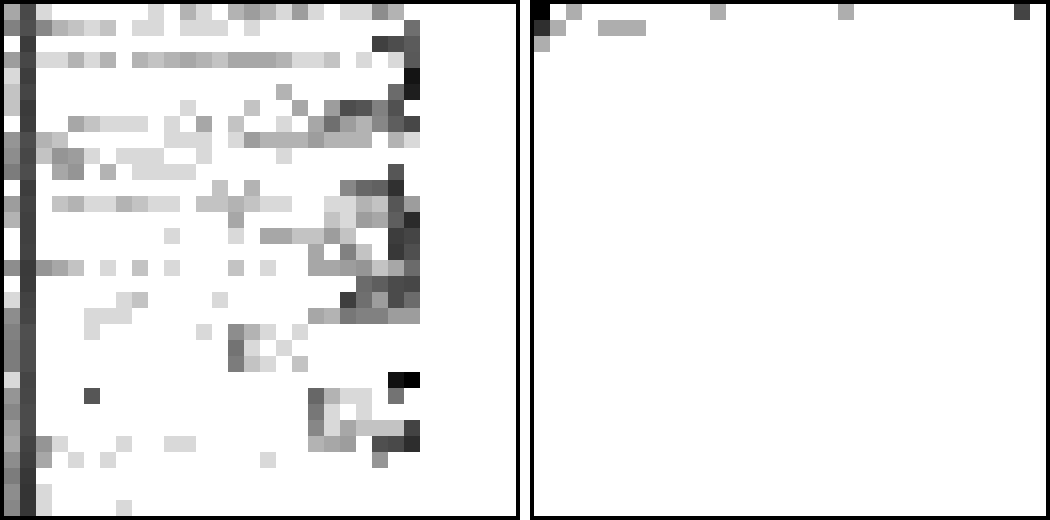
\includegraphics[width=0.6\textwidth]{obrazky-figures/10_m22_flowpics.png}
	\caption{FlowPic reprezentace vytvořené z~dvou náhodně vybraných toků z~datové sady Mirage22 s~filtrem >10pkts.}
	\label{10_m22_flowpic}
\end{figure}

\begin{figure}[H]
	\centering
	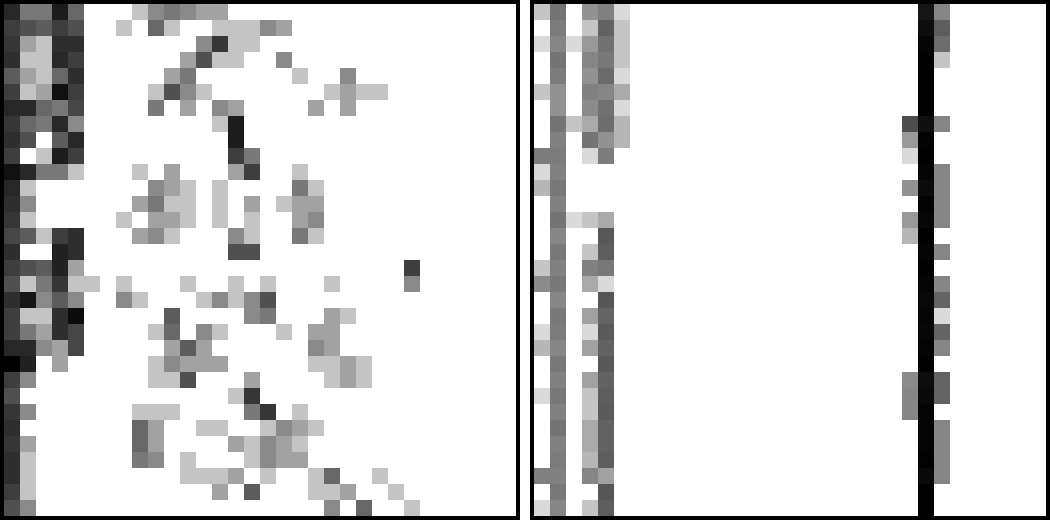
\includegraphics[width=0.6\textwidth]{obrazky-figures/1000_m22_flowpics.png}
	\caption{FlowPic reprezentace vytvořené z~dvou náhodně vybraných toků z~datové sady Mirage22 s~filtrem >1\,000pkts.}
	\label{1000_m22_flowpic}
\end{figure}

Oproti datové sadě Mirage19 lze pozorovat, že výsledné FlowPic reprezentace jsou mnohem plnější a~bohatší. To umožní dosáhnout výraznějších rozdílů mezi augmentovanými vzorky, což povede k~lepší generalizaci modelu.

\subsection{Ucdavis-icdm19}
\label{ucdavis_section}
Dataset ucdavid-icdm19 obsahuje zachycený provoz z~pěti služeb společnosti Google. Konkrétně se jedná o~služby Google Drive, Youtube, Google Docs, Google Search a~Google Music. Dataset obsahuje 6\,672 vzorků. Celkový počet tříd činí 5~\cite{usdavis}.

Tato datová sada se od ostatních odlišuje tím, že pro testování modelu nabízí dvě testovací části, \textit{human} a~\textit{script}, které se liší od té využívané pro trénování. Část \textit{script} je generována skripty a~automatizovanými nástroji, zatímco \textit{human} zachycuje provoz reálných uživatelů.

\begin{table}[H]
    \centering
    \resizebox{\textwidth}{!}{%
        \begin{tabular}{l c c c c c c c}
            \toprule
            \textbf{Název} & \textbf{Rozdělení} & \textbf{Filtry} & \textbf{Třídy} & \textbf{Počet toků} &  \makecell{\textbf{Průměrná délka}\\ \textbf{toku}} & \makecell{\textbf{Průměrný počet}\\ \textbf{paketů}} \\
            \midrule
           \multirow{4}{*}{Ucdavis-icdm19} 
              & pretraining & \multirow{4}{*}{\centering\makecell{žádný}} & \multirow{4}{*}{5} & 6\,439 & 42,92\,s & 6\,652,93\\
              & val   &  & & 1\,288 & 43,50\,s & 6\,811,09\\
              & human  &  & & 83 & 31,33\,s & 7\,666,37\\
              & script  &  & & 150 & 42,94\,s & 7\,130,64\\
            \bottomrule
        \end{tabular}
    }
    \caption{Analýza datové sady Ucdavis-icdm19.}
    \label{ucdavis_analysis}
\end{table}

\begin{figure}[H]
	\centering
	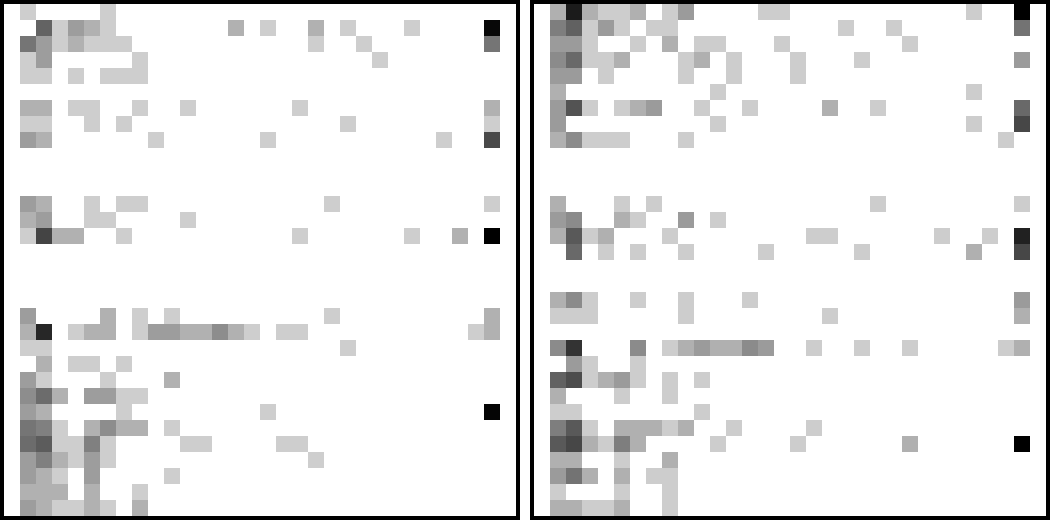
\includegraphics[width=0.6\textwidth]{obrazky-figures/ucd_flowpics.png}
	\caption{FlowPic reprezentace vytvořené z~dvou náhodně vybraných toků z~datové sady Ucdavis-icdm19.}
	\label{ucd_flowpics}
\end{figure}

\begin{figure}[H]
	\centering
	
\includegraphics[width=0.6\textwidth]{obrazky-figures/script_human_flowpics.png}
	\caption{Porovnání FlowPic reprezentací vytvořených z~části \textit{script} (vlevo) a~\textit{human} (vpravo).}
	\label{ucd_h_s_flowpics}
\end{figure}

Na vytvořených FlowPic reprezentacích můžeme pozorovat velice dobrou distribuci paketů napříč FlowPicem. Augmentace aplikované na tyto reprezentace tak budou mnohem výraznější než u~prázdnějších FlowPiců, což může vést k~lepší generalizaci modelu.

\subsection{UTMobileNetTraffic2021}
Dataset obsahuje více než 29 hodin síťového provozu generovaného jak automatizovanou platformou, tak lidskými uživateli. Zachycený provoz pochází z~16 nejoblíbenějších mobilních aplikací, jako jsou Reddit, Spotify, YouTube, Instagram, Hulu a~další. Celkem tento dataset obsahuje 9\,460 vzorků a~celkový počet tříd činí 14~\cite{UTMobileNetTraffic}.

\begin{table}[H]
    \centering
    \resizebox{\textwidth}{!}{%
        \begin{tabular}{l c c c c c c c}
            \toprule
            \textbf{Název} & \textbf{Rozdělení} & \textbf{Filtry} & \textbf{Třídy} & \textbf{Počet toků} &  \makecell{\textbf{Průměrná délka}\\ \textbf{toku}} & \makecell{\textbf{Průměrný počet}\\ \textbf{paketů}} \\
            \midrule
            \multirow{3}{*}{UTMobileNetTraffic2021} 
              & train & \multirow{3}{*}{\centering\makecell{žádný}} & \multirow{3}{*}{14} & 7\,568 & 13,47\,s & 2\,537,27\\
              & val   &  &  & 946 & 67,40\,s & 1\,554,43\\
              & test  &  &  & 946 & 1,59\,s & 1\,810,65\\
            \bottomrule
        \end{tabular}
    }
    \caption{Analýza datové sady UTMobileNetTraffic2021 bez filtru.}
    \label{utmob_no_filter}
\end{table}

\begin{table}[H]
    \centering
    \resizebox{\textwidth}{!}{%
        \begin{tabular}{l c c c c c c c}
            \toprule
            \textbf{Název} & \textbf{Rozdělení} & \textbf{Filtry} & \textbf{Třídy} & \textbf{Počet toků} &  \makecell{\textbf{Průměrná délka}\\ \textbf{toku}} & \makecell{\textbf{Průměrný počet}\\ \textbf{paketů}} \\
            \midrule
            \multirow{3}{*}{UTMobileNetTraffic2021} 
              & train & \multirow{3}{*}{\centering\makecell{$>$30pkts}} & \multirow{3}{*}{14} & 5\,028 & 18,23\,s & 3\,808,52\\
              & val   &  & & 656 & 93,25\,s & 2\,232,41\\
              & test  &  & & 648 & 1,05\,s & 2\,633,73\\
            \bottomrule
        \end{tabular}
    }
    \caption{Analýza datové sady UTMobileNetTraffic2021 s~filtrem >30pkts.}
    \label{utmob_filter}
\end{table}

Podobně jako u~datové sady Mirage19 je i~zde zvolen větší filtr než v~referenční práci~\cite{huawei_paper} z~důvodu absence toků kratších než 10 paketů.

\begin{figure}[H]
	\centering
	
\includegraphics[width=0.6\textwidth]{obrazky-figures/utm_flowpics.png}
	\caption{FlowPic reprezentace vytvořené z~dvou náhodně vybraných toků z~datové sady UTMobileNetTraffic2021 bez filtru.}
	\label{utm_flowpics}
\end{figure}

\begin{figure}[H]
	\centering
	
\includegraphics[width=0.6\textwidth]{obrazky-figures/f_utm_flowpics.png}
	\caption{FlowPic reprezentace vytvořené z~dvou náhodně vybraných toků z~datové sady UTMobileNetTraffic2021 s~filtrem.}
	\label{f_utm_flowpics}
\end{figure}

Podobně jako u~datové sady Mirage19 můžeme pozorovat velmi špatnou distribuci paketů. Tedy i~tato datová sada nemůže dosahovat dobrých výsledků.

\subsection{CESNET}
\label{cesnet_dat}
Poslední datová sada byla vytvořena sdružením CESNET\footnote{\url{https://www.cesnet.cz/}}. Jedná se o~největší dataset ze všech použitých, a~tedy obsahuje i~nejvyšší počet síťových toků. Jeho celková velikost přesahuje 7,1\,GB. Vzhledem k~tomu, že cílem je využít tuto sadu výhradně pro tvorbu \textit{embeddingů}, tedy pro kontrastivní učení, bude nasazena v~kombinaci s~ostatními datovými sadami.

\begin{table}[H]
    \centering
    \resizebox{\textwidth}{!}{%
        \begin{tabular}{l c c c c c c c}
            \toprule
            \textbf{Název} & \textbf{Rozdělení} & \textbf{Filtry} & \textbf{Třídy} & \textbf{Počet toků} &  \makecell{\textbf{Průměrná délka}\\ \textbf{toku}} & \makecell{\textbf{Průměrný počet}\\ \textbf{paketů}} \\
            \midrule
            CESNET & žádné & žádné & 15 & 590\,962 & 70,00\,s & 519,20 \\
            \bottomrule
        \end{tabular}
    }
    \caption{Analýza datové sady CESNET.}
    \label{utmob_filter}
\end{table}

\begin{figure}[H]
	\centering
	
\includegraphics[width=0.6\textwidth]{obrazky-figures/cesnet_flowpics4.png}
	\caption{FlowPic reprezentace vytvořené z~dvou náhodně vybraných toků z~datové sady CESNET.}
	\label{cesnet_dataset}
\end{figure}

Vytvořené FlowPic reprezentace se výrazně podobají těm z~datových sad Mirage19, Mirage22 a~UTMobileNetTraffic21. Aplikace časového filtru, který by odstraňoval toky kratší než nějaká zvolená délka, v~tomto případě nebude efektivní, neboť značná část paketů přichází již během první sekundy komunikace. Výhodou této nové datové sady však může být její rozsah, vysoký počet toků totiž může do určité míry kompenzovat nízkou kvalitu FlowPic reprezentací.

%=====================================================================================%
\section{Model}
Tato práce si klade za cíl replikovat výsledky dosažené v~\cite{flowpic_augmentations}. Model použitý v~této práci je proto odvozen od modelu prezentovaného v~práci referenční.

\subsection{Příprava dat}
Framework \textit{SimCLR} generuje dva augmentované pohledy $\tilde{x}_i$ a~$\tilde{x}_j$ pomocí různých náhodných augmentací, které jsou popsány v~sekci~\ref{augmentace}, jež budou tvořit pozitivní pár. Tyto pohledy jsou následně použity k~vytvoření FlowPic reprezentací.

Vzhledem k~výpočetní náročnosti standardně velkých FlowPic reprezentací o~rozměrech 1\,500$\times$1\,500, popsaných v~sekci~\ref{flowpic_text}, bude v~této práci použita jejich zmenšená verze nazvaná mini-FlowPic, která je detailně popsána v~sekci~\ref{mini_flowpics}. Konkrétně bude použita velikost 32$\times$32. Standardní FlowPic mapuje velikost paketu v~poměru 1:1 na ose $Y$ (do maximální MTU), zatímco menší verze používá transformaci, která je podrobněji popsána v~sekci~\ref{mini_flowpics}. Osa $X$ v~obou případech reprezentuje čas.

\subsection{Extrakce reprezentací}
\label{extrakce}
Extrakce reprezentací je část, kde se bude využívat kontrastivní učení společně s~\textit{SimCLR} frameworkem.

Klíčovou komponentou v~této fázi je CNN, která je v~sekci~\ref{CNNs} teoreticky popsána, a~v rámci \textit{SimCLR} je označována jako $f(\cdot)$. Podobně jako v~pracích~\cite{flowpic_augmentations}~a~\cite{FlowPic}, i~zde vychází základní architektura z~modelu LeNet-5~\cite{lenet5}.
\begin{figure}[H]
	\centering
	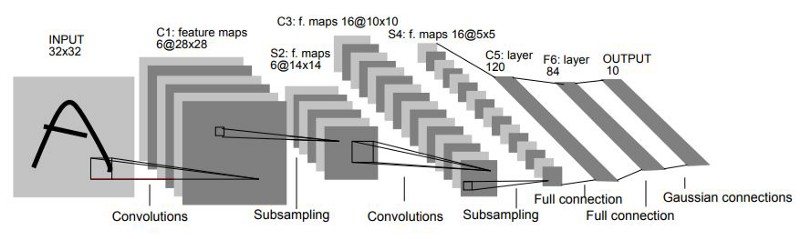
\includegraphics[width=1\textwidth]{obrazky-figures/lenet5.jpeg}
	\caption{LeNet-5 architektura~\cite{lenet5}.}
	\label{lenet5_architektura}
\end{figure}

Původní LeNet-5 architekturu, popsanou na obrázku~\ref{lenet5_architektura}, je potřeba pro účely této fáze upravit. V~původním modelu jsou vrstvy S2 a~S4 implementovány jako \textit{pooling} vrstvy využívající průměrování, tedy tzv. \textit{average pooling}, ovšem dle referenční práce~\cite{flowpic_augmentations} je vhodnější využít výběr maxima (tzv. \textit{max pooling}). Další modifikací je nahrazení posledních dvou vrstev (F6 a~OUTPUT) dvěma lineárními vrstvami o~velikosti 120 a~30. Tímto získáme 120 dimenzionální vektor $h~=~f(FlowPic)$ a~30 dimenzionální vektor podobnosti $z = g(h)$. Pro trénink bude využita ztrátová funkce, která je popsána v~sekci~\ref{loss_func}.
\begin{figure}[H]
	\centering
	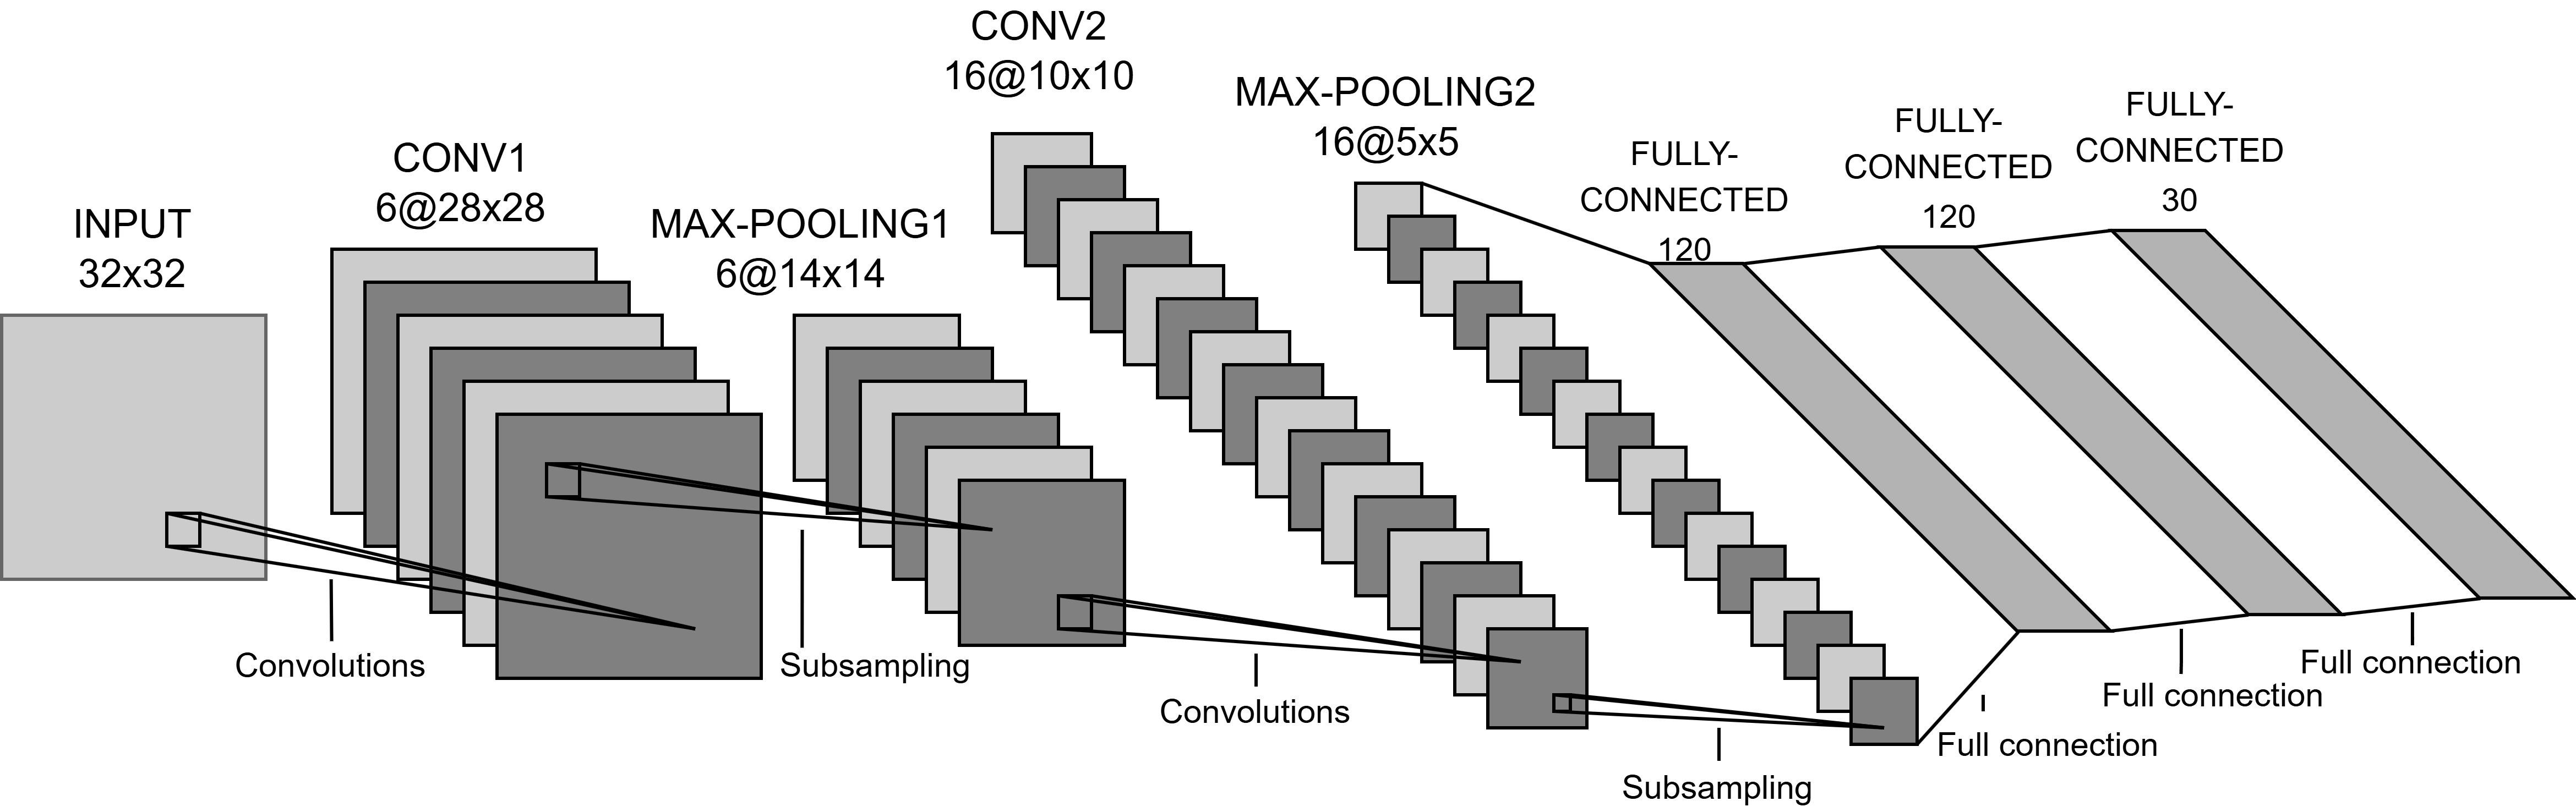
\includegraphics[width=1\textwidth]{obrazky-figures/custom_cnn.png}
	\caption{Ilustrace architektury pro 32$\times$32 Mini FlowPic.}
	\label{proposed_architektura}
\end{figure}

\subsection{Lineární klasifikátor}
\label{lin_classifier}
Jako možnost zhodnocení naučených reprezentací je zvolen lineární klasifikátor, který je trénován na klasifikaci vektorů reprezentací. Extrakce, popsaná v~sekci~\ref{extrakce}, byla prováděna jako učení bez učitele (tzv. \textit{unsupervised learning}), nicméně tento lineární klasifikátor bude trénován s~učitelem (tzv. \textit{supervised learning}), tj. s~pomocí označených vzorků. v~této fázi se zmrazí váhy využívané při trénování $f(\cdot)$, což znamená že extraktor se stane fixním extraktorem reprezentací, aby bylo možné lineární klasifikátor efektivně trénovat.

Lineární klasifikátor je jednoduchá, jednovrstevná neuronová síť, která může být popsaná vzorcem $y = xA^{T} + b$, kde $A$, $b$ jsou klasifikační parametry, $x$ je vstupní vektor a~$y$ je výstupem. Jak popisuje sekce~\ref{extrakce}, vstupní vektor $x$ je 120 dimenzionální.
%=====================================================================================%
\section{Návrh experimentů}
\label{training_proposal}
Toky z~vybraných datových sad budou načítány pomocí dataloaderů z~knihovny FlowMind. V~souladu s~frameworkem SimCLR, popsaným v~sekci~\ref{simclr_text}, bude každý tok duplikován, aby na něj mohla být následně aplikována augmentace. Zvolené augmentační techniky, uvedené v~sekci~\ref{augmentace}, budou, s~výjimkou rotace FlowPic reprezentace, aplikovány přímo na samotný tok před konstrukcí výsledného FlowPicu. Rotace jako jediná proběhne až po vytvoření reprezentace.
Pro každý pozitivní pár bude použita tatáž augmentační technika, lišící se pouze v~konkrétních hodnotách parametrů, které budou náhodně vybírány z~předem definovaných intervalů. Tyto intervaly jsou navrženy tak, aby umožnily srovnání dosažených výsledků s~referenčními pracemi~\cite{flowpic_augmentations} a~\cite{huawei_paper}. Konkrétně bude hodnota $\alpha$ pro modifikaci RTT vybírána z~intervalu [0,5; 1,5], zatímco hodnota $b$ pro časový posun při modifikaci IAT bude náhodně zvolena z~rozsahu [-1,0; 1,0]. Augmentace vynechání paketů bude pracovat s~$\Delta t = 0{,}1$ a~náhodně určeným časovým bodem $t$ v~intervalu [0; délka toku]. Poslední augmentací je rotace FlowPic reprezentace, která se bude pohybovat v~rozmezí [-10$^\circ$; 10$^\circ$].

Při učení bez učitele jsou výsledné FlowPic reprezentace využívány k~trénování jak CNN \textit{encoderu} $f(\cdot)$, tak projekční hlavy $g(\cdot)$. Cílem je získat kvalitní \textit{embeddingy}, které mohou být předány ztrátové funkci. Na základě zpětné propagace se následně aktualizují váhy obou těchto částí modelu. Po ukončení tohoto trénovacího procesu následuje \textit{fine-tuning} (fáze učení s~učitelem), při kterém je \textit{encoder} zmrazen, tedy jeho váhy zůstávají beze změny. Původní projekční hlava $g(\cdot)$ je odstraněna a~nahrazena novou klasifikační hlavou (lineárním klasifikátorem), která je jako jediná část modelu aktivně trénována a~optimalizována na základě dat, která zatím nebyla pro trénování použita. V~kontextu této práce se jedná o~testovací části datových sad. Rozdílem mezi projekční hlavou a~klasifikační hlavou je také jejich výstup. Zatímco projekční hlava produkuje třicetidimenzionální vektor podobnosti $z$, klasifikační hlava se snaží výsledky mapovat na jednotlivé třídy.

Celý proces trénování, zahrnující jak učení bez učitele, tak učení s~učitelem, bude zopakován celkem pětkrát a~výsledky budou průměrovány. Pro širší kontext bude také uvedena směrodatná odchylka mezi výsledky. Důvodem je skutečnost, že hodnoty jednotlivých augmentací jsou vybírány náhodně a~výsledky se tak mohou mírně lišit.

\begin{figure}[H]
	\centering
	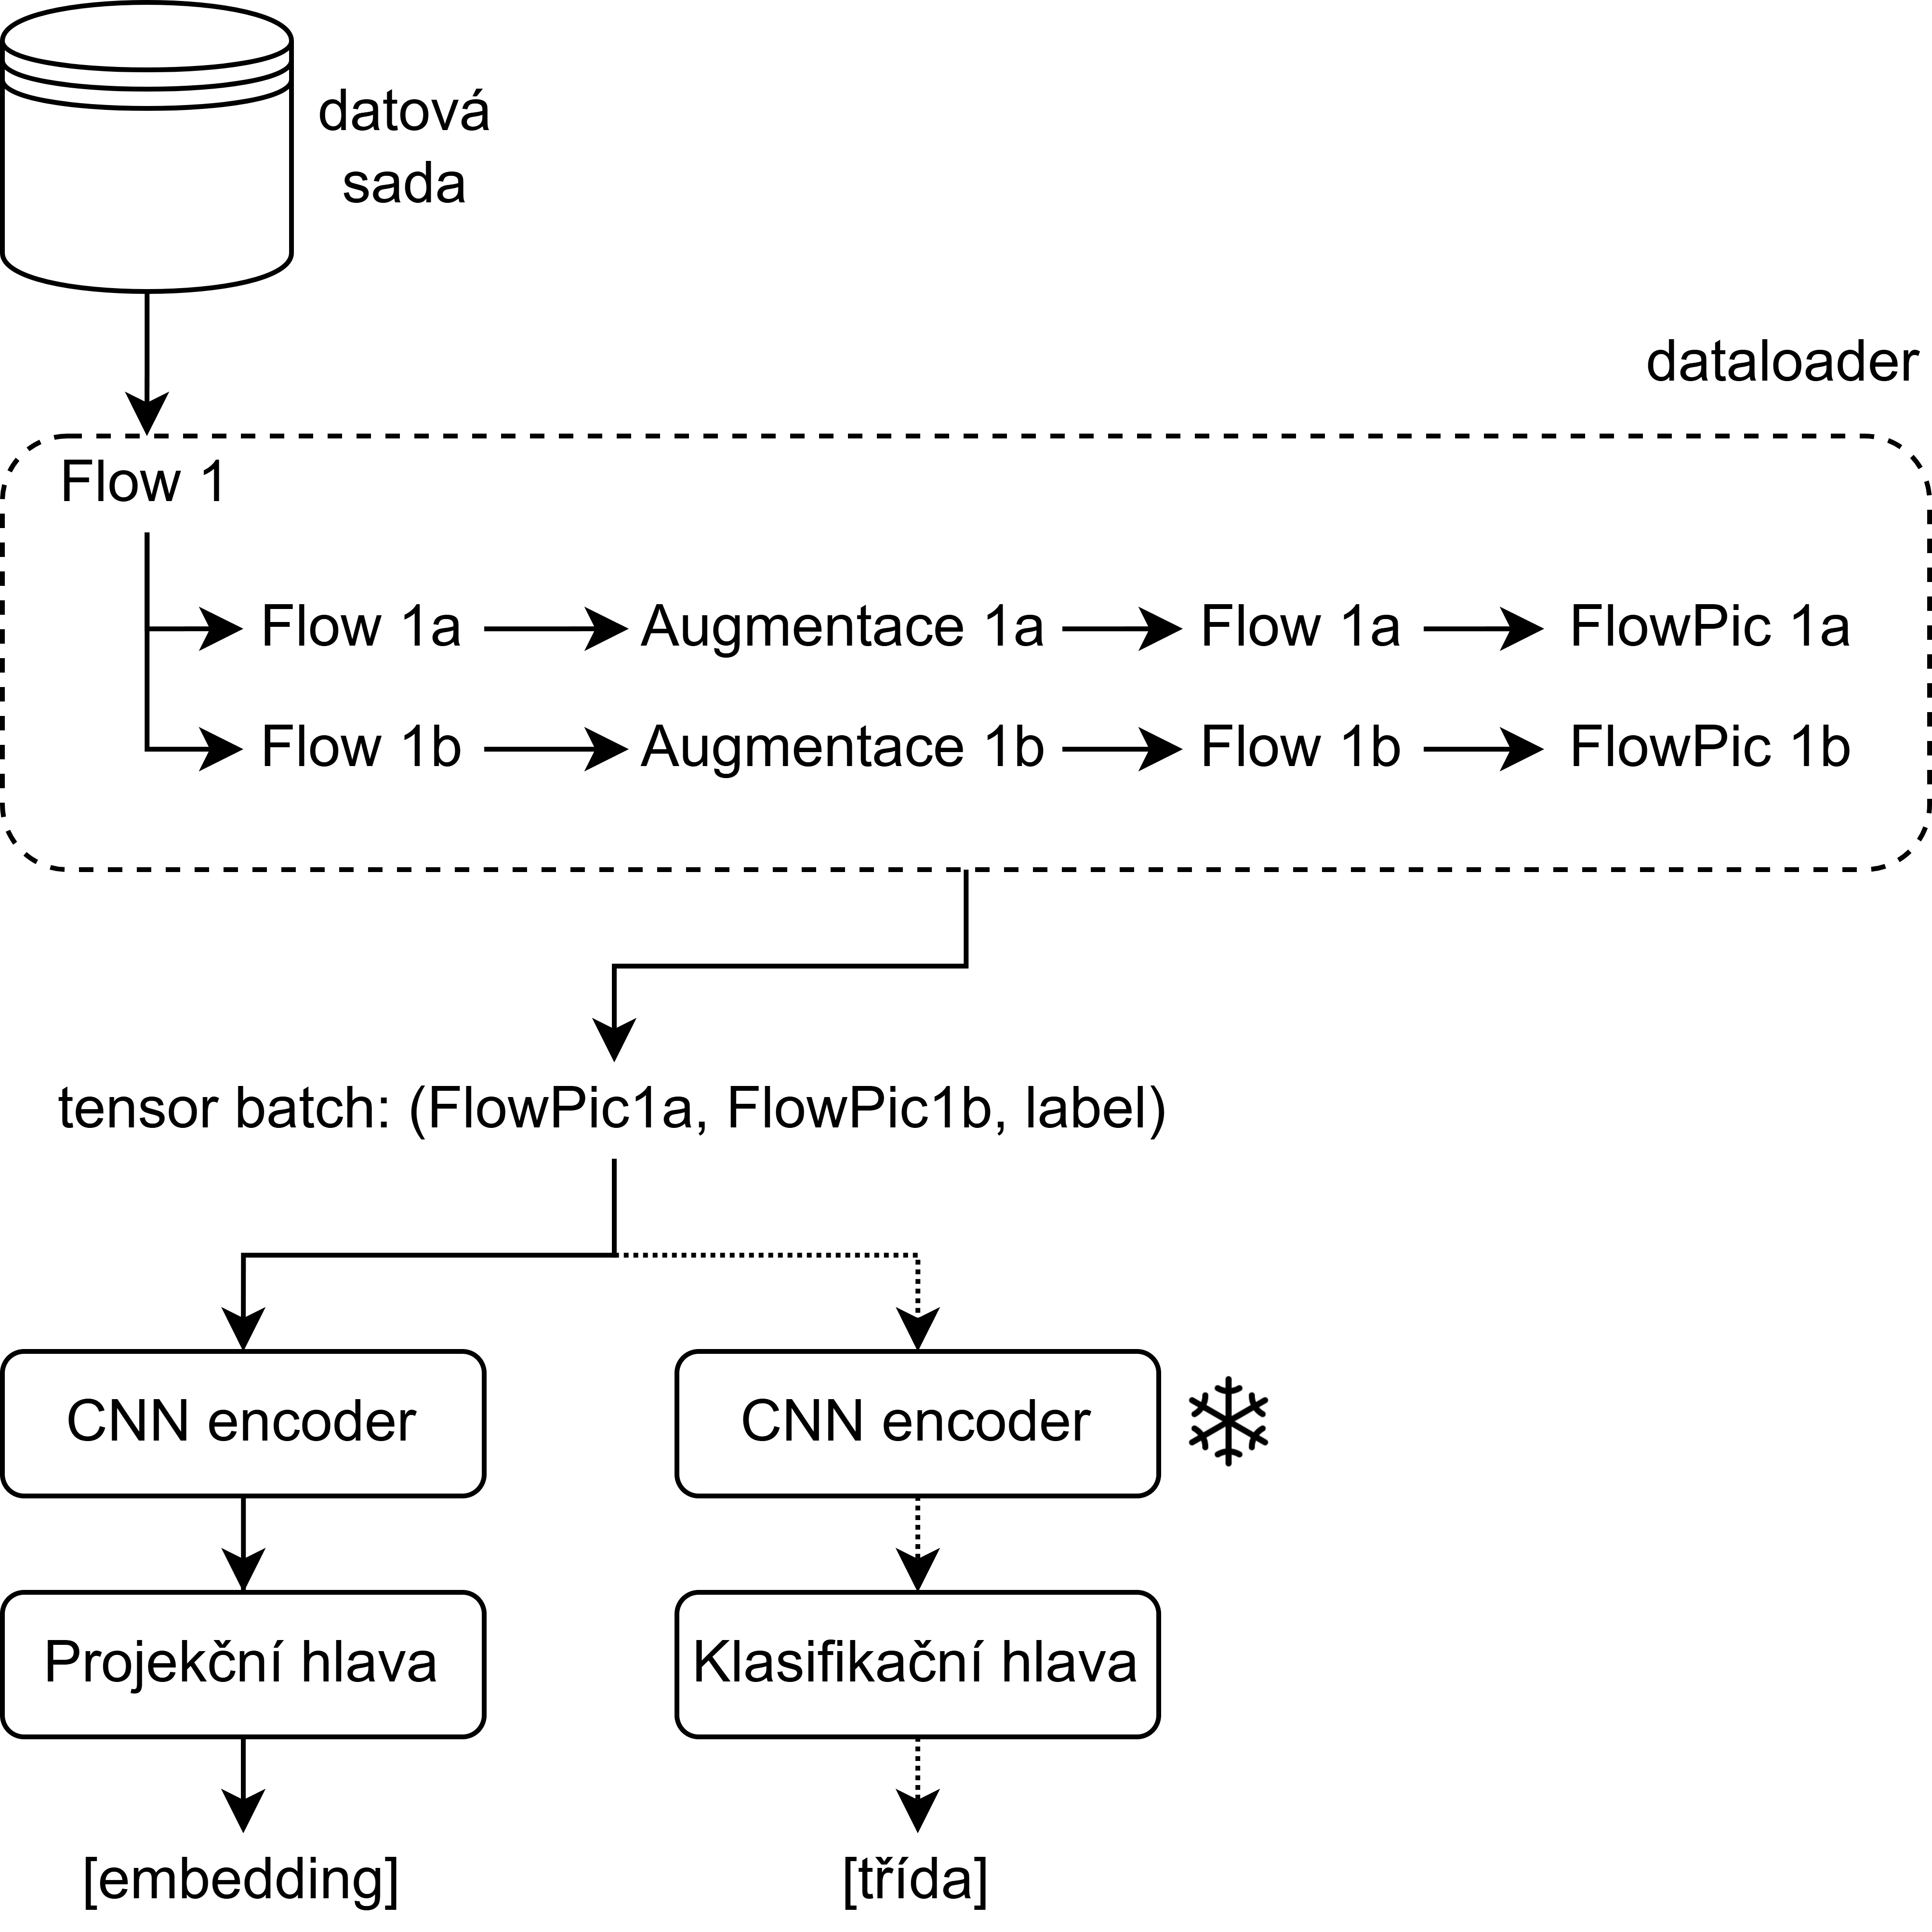
\includegraphics[width=0.7\textwidth]{obrazky-figures/training.png}
	\caption{Ilustrace procesu trénování. Sněhová vločka značí zmražení \textit{encoderu}.}
	\label{training_diagram}
\end{figure}

%=====================================================================================%
%=====================================================================================%
\chapter{Implementace a~vyhodnocení dosažených výsledků}
Tato kapitola popisuje zvolenou implementaci, výběr hyperparametrů a~postup trénování neuronové sítě. Z~vybraných datových sad, které jsou v~této práci pro trénink modelu zvoleny, využívá referenční práce~\cite{flow_monitoring} pouze jednu, konkrétně Ucdavis-icdm19~\cite{usdavis}, popsanou v~sekci~\ref{ucdavis_section}. Z~tohoto důvodu budou výsledky na ostatních datových sadách porovnávány s~výsledky dosažených v~práci~\cite{huawei_paper}, která práci referenční rozšiřuje o~další datové sady.

Pro verzování kódu a dokumentace byl využit GitHub repozitář\footnote{\url{https://github.com/Simkuba/IBT}}.

%=====================================================================================%
\section{Použité knihovny}
Tato sekce se zaměřuje na knihovny, které byly využity při implementaci neuronové sítě a~všech souvisejících komponent. Obě zmíněné knihovny jsou pro tuto práci esenciální. Kromě jejich popisu tato sekce zároveň demonstruje implementaci jednotlivých částí neuronové sítě.

\subsection{PyTorch}
Pro implementaci konvoluční neuronové sítě i~lineárního klasifikátoru byla využita knihovna PyTorch\footnote{\url{https://pytorch.org/}}, což je velmi bohatá knihovna, která poskytuje četné funkce umožňující vytváření stavebních bloků pro hluboké učení. Knihovna poskytuje základní datovou strukturu \textit{tensor}, což není nic jiného než vícerozměrné pole objektů stejného typu. Lze říci, že na nižší úrovni abstrakce jsou veškeré výpočty v~PyTorch založeny na tensorech a~operacích nad nimi~\cite{pytorch}.

Konkrétněji je \textit{tensor} zobecněný způsob reprezentace skalárů, vektorů a~matic, který lze definovat jako n-rozměrnou matici. 0-rozměrný \textit{tensor} (tj. jedno číslo) se nazývá skalár, 1-rozměrný se nazývá vektor, 2-rozměrný se nazývá matice a~3-rozměrný se také označuje jako krychle~\cite{pytorch}. 

V~této práci je pro ukládání dat využíván 4D (tedy. čtyřrozměrný) \textit{tensor} ve formátu [B,~C,~H,~W], kde B~označuje velikost batche (tzv. \textit{batch size}), C~označuje počet kanálů, H~označuje výšku FlowPicu a~W~jeho šířku. Ve všech případech trénování (pokud není uvedeno jinak) je využito [32,~1,~32,~32], tedy \textit{batch size} 32, 1~kanál a~velikost FlowPicu~32x32.

\subsubsection*{Implementace CNN}
PyTorch nabízí předpřipravené třídy pro implementaci konvolučních neuronových sítí, což výrazně zjednodušuje jejich vytváření. Vzhledem k~rozměrům \textit{tensorů} používaných v~této práci je vhodné využívat 2d varianty těchto tříd, které jsou navrženy pro práci se 4D \textit{tensory}. Konkrétně jsou využity třídy \texttt{nn.Conv2d()}, \texttt{nn.BatchNorm2d()} a~\texttt{nn.MaxPool2d()}. Výsledný \textit{encoder} $f(\cdot)$ poté ještě obsahuje jednu lineární vrstvu, která je implementována pomocí třídy \texttt{nn.Linear()}. Aktivační \textit{ReLU} funkce je implementována pomocí třídy \texttt{nn.ReLU()}. Všechny tyto vrstvy lze obalit třídou \texttt{nn.Sequential()}, což je kontejnerová třída, která umožňuje řetězit více vrstev dohromady v~přesném pořadí, v~jakém jsou zapsané. 

Implementace výsledného \textit{encoderu} $f(\cdot)$ tedy vypadá následovně:
\begin{lstlisting}[caption={Implementace \textit{encoderu} $f(\cdot)$.}]
nn.Sequential(
    nn.Conv2d(in_channels=1, out_channels=6, kernel_size=5),
    nn.BatchNorm2d(6),
    nn.ReLU(),
    nn.MaxPool2d(kernel_size=2, stride=2),
        
    nn.Conv2d(in_channels=6, out_channels=16, kernel_size=5),
    nn.BatchNorm2d(16),
    nn.ReLU(),
    nn.MaxPool2d(kernel_size=2, stride=2),
        
    nn.Flatten(),
    nn.Linear(400, 120),
    nn.ReLU(),
)
\end{lstlisting}

Implementace \textit{encoderu} tedy vychází z~referenční práce~\cite{flowpic_augmentations}. Navíc jsou ovšem přidané normalizační vrstvy \texttt{nn.BatchNorm2d}, jelikož bylo v~průběhu trénování pozorováno, že mají pozitivní vliv na výsledné reprezentace a~tedy i~na konečnou přesnost modelu.

\subsubsection*{Implementace projekční hlavy}
V~rámci frameworku SimCLR navazuje na \textit{encoder} $f(\cdot)$ projekční hlava $g(\cdot)$, která se využívá k~získání třicetidimenzionálního vektoru podobnosti $z = g(h)$. Projekční hlava obsahuje pouze lineární vstvy implementované pomocí třídy \texttt{nn.Linear()}. Nově se zde využívá také \textit{Tanh} aktivační funkce implementována pomocí třídy \texttt{nn.Tanh()}.
\begin{lstlisting}[caption={Implementace projekční hlavy $g(\cdot)$.}]
nn.Sequential(
    nn.Linear(120,120),
    nn.ReLU(),
    nn.Linear(120,30),
    nn.Tanh()
)
\end{lstlisting}

\subsubsection*{Implementace lineárního klasifikátoru}
Jak je popsáno v~sekci~\ref{lin_classifier}, lineární klasifikátor používaný pro tzv. \textit{fine-tuning} je jednoduchá jednovrstevná neuronová síť. Z~toho důvodu ji ani není potřeba obalovat kontejnerovou vrstvou \texttt{nn.Sequential()} a~lze ji implementovat jednou třídou \texttt{nn.Linear()}. Vstupem je 120-dimenzionální vektor a~výstupem je vektor o~velikosti počtu tříd, který se liší podle použité datové sady.

\subsection{FlowMind}
K~načítání dat z~datových sad a~jejich převodu do FlowPic reprezentací byla využita knihovna FlowMind, vyvíjená na Fakultě informačních technologií Vysokého učení technického v~Brně. Pro tzv. \textit{dataloader}, který zajišťuje načtení a~následné zpracování dat, byla použita funkce \texttt{create\_flowpic\_dataloader()}. Tato funkce byla pro účely kontrastivního učení mírně upravena tak, aby místo jediné FlowPic reprezentace vracela tensor obsahující dvě. Za tímto účelem byla knihovna rozšířena o~funkci \texttt{build\_two\_augmented\_flows()}, která toto chování implementuje.

Proces zpracování dat pomocí funkce \texttt{create\_flowpic\_dataloader()} je poměrně přímočarý. Funkce, kromě dalších argumentů, přijímá cestu k~datové sadě, jejíž jednotlivé toky postupně zpracovává. Toky jsou nejprve převedeny z~formátu \texttt{.csv} do Python datové struktury \textit{dictionary}, následně jsou filtrovány na základě počtu paketů či délky toku, a~poté je každý tok duplikován a~předán již zmíněné funkci \texttt{build\_two\_augmented\_flows()}. Ta následně pomocí dalších tříd definovaných v~knihovně FlowMind vytvoří dvě augmentované FlowPic reprezentace.

Pomocí \textit{dataloaderu} jsou na jednotlivé toky také aplikovány vybrané augmentace, které jsou podrobně popsány v~sekcích~\ref{augmentace} a~\ref{training_proposal}. Všechny z~nich, s~výjimkou rotace FlowPicu, se aplikují přímo na síťový tok ještě před samotnou konstrukcí FlowPic reprezentace. K~provádění těchto úprav slouží parametry \texttt{flow\_transform1} a~\texttt{flow\_transform2}, jenž se dále předávají až ke třídě odpovědné za konstrukci samotného toku, tedy objektu \texttt{Flow}. Naproti tomu augmentace rotace FlowPicu se neprovádí prostřednictvím \textit{dataloaderu}, ale aplikuje se až na vytvořenou FlowPic reprezentaci v~rámci tréninkové smyčky.

Pro korektní načtení dat a~sestavení FlowPic reprezentace je u~\textit{dataloaderu} nutné definovat několik klíčových parametrů. Mezi nimi je klíčové slovo \texttt{meta\_key}, které slouží k~určení, podle čeho budou sestavovány \textit{labely}, dále cesta k~datové sadě, hodnota \textit{batch size}, časový interval [0; 15], určující prvních patnáct sekund toku, a~velikostní interval [0; 1\,500], kde hodnota 1\,500 odpovídá MTU (\textit{Maximum Transmission Unit}). Dále je třeba nastavit parametr \texttt{bidirectional} na hodnotu \texttt{False}, aby tensor obsahoval pouze jeden kanál. Nakonec se předává parametr \texttt{dp\_transform}, který zajišťuje transformaci \textit{labelu} na číselnou hodnotu.

Knihovna rovněž poskytuje implementaci ztrátové funkce NT-Xent, která je matematicky ověřená a~byla využita ve fázi učení bez učitele.
%=====================================================================================%

\section{Postup trénování}
Pro trénování byly hyperparametry nastaveny tak, aby bylo možné dosažené výsledky porovnávat s~referenčními prácemi~\cite{flowpic_augmentations} a~\cite{huawei_paper}. 

Pro trénování bez učitele (\textit{unsupervised learning}) byl nastaven \textit{learning rate} na hodnotu 0,001, jako ztrátová funkce byla využita NT-Xent Loss, popsaná v~sekci~\ref{loss_func}, s~teplotním parametrem 0,07. Jako optimalizační algoritmus byl zvolen Adam, který patří mezi metody využívající výpočet gradientu. Samotné trénování využívalo předčasné ukončení (\textit{early stopping}), které sledovalo vývoj ztrátové funkce na validačním setu s~maximální trpělivostí (\textit{patience}) 3, přičemž maximální počet epoch byl omezen na 30.

Pro \textit{fine tuning}, tedy trénování s~učitelem, byla hodnota \textit{learning rate} nastavena na 0,01, pro ztrátovou funkci byla využita \textit{Cross-Entropy Loss}. Jako optimalizační algoritmus byl, stejně jako při trénování bez učitele, zvolen Adam. Přesnost modelu se počítala pomocí PyTorch třídy \texttt{MultiClassAccuracy}. Také zde bylo využito předčasné ukončení, které sledovalo minimální zlepšení modelu s~hodnotou 0,001 a~trpělivostí~5. Celkový počet epoch byl omezen na 20.

Všechny datové sady, s~výjimkou CESNET popsaného v~sekci~\ref{cesnet_dat}, jsou rozděleny na části \textit{train}, \textit{val} a~\textit{test}, přičemž každá z~nich slouží k~jiné fázi učení. Datová sada Ucdavis-icdm19, popsaná v sekci~\ref{ucdavis_section}, dokonce obsahuje 2 testovací části, \textit{human} a~\textit{script}. Část \textit{train} je určena pro trénování CNN a~zároveň se na ni aplikují augmentace. Stejná část je, opět s~výjimkou datasetu CESNET, využita i~při \textit{fine-tuningu}, avšak již bez aplikování augmentací. Část \textit{val} slouží k~validaci modelu během trénování a~jsou na ni aplikovány stejné augmentace jako na trénovací sadu. Poslední částí je \textit{test}, která slouží k~ověření výsledné přesnosti modelu. Vzhledem k~již zmíněným odlišnostem datové sady Ucdavis-icdm19 je model testován samostatně jak proti celé části \textit{human}, tak i~proti celé části \textit{script}, a~tedy celkově testován dvakrát.

Jednotlivé smyčky jsou implementovány pomocí čtyř funkcí. Liší se tím, jaká část datové sady je právě využívána a~jakým způsobem je model trénován. Trénovací smyčka nastaví model do trénovacího módu pomocí PyTorch metody \texttt{train()}. Z~\textit{dataloaderu} jsou postupně vybírány dvojice FlowPic reprezentací, které jsou následně předány modelu. Po získání vektorů $z_{1}$ a~$z_{2}$ je vypočítána ztrátová funkce a~aktualizují se váhy. 

Validační smyčka se od trénovací liší tím, že celý proces, tedy akce probíhající v~trénovací smyčce, je zabalen do PyTorch kontextového manažeru \texttt{torch.no\_grad()}, který během svého trvání (v~bloku \texttt{with}) vypne výpočet gradientů. Model je zároveň nastaven do evaluačního módu pomocí PyTorch metody \texttt{eval()}. V~samotné validační smyčce se oproti trénovací již model neoptimalizuje, tedy váhy zůstávají nezměněné. Důvodem je to, že validační smyčka slouží pouze k~vyhodnocení modelu, nikoli k~jeho trénování.

Třetí je klasifikační smyčka, která je použita při učení s~učitelem. Jelikož se jedná o~fázi tzv. \textit{fine-tuningu}, je nutné \textit{encoder} $f(\cdot)$ zmrazit. Toho je dosaženo nastavením atributu tenzorů \texttt{requires\_grad} na hodnotu \texttt{False}. Ve smyčce je také odstraněna projekční hlava $g(\cdot)$ CNN modelu a~nahrazena lineárním klasifikátorem (MLP modelem). Oba modely musí být náležitě nastaveny, tedy CNN model je přepnut do evaluačního módu pomocí \texttt{eval()} a~MLP model do trénovacího módu \texttt{train()}. Dalším rozdílem je také použití jiné ztrátové funkce.

Poslední smyčkou je testovací smyčka, která nastavuje oba modely do evaluačního módu \texttt{eval()} a~stejně jako validační smyčka využívá kontextový manažer \texttt{torch.no\_grad()}.

Celý proces trénování byl zopakován v~pěti bězích u~každé datové sady, přičemž uváděné přesnosti představují průměrné hodnoty napříč všemi běhy. U~každé hodnoty je uvedena také směrodatná odchylka.

%=====================================================================================%
\section{Dosažené výsledky}
Tato sekce prezentuje výsledky dosažené na vybraných datových sadách popsaných v~sekci~\ref{datasets}. Hodnoty jsou uváděny pro jednotlivé typy augmentací, aby bylo možné je mezi sebou porovnat. Vzhledem k~povaze některých datových sad jsou u~vybraných případů prezentovány výsledky bez i~s~aplikovaným filtrováním. Kde je to možné, jsou výsledky této práce porovnány s~výsledky dosaženými v~referenčních studiích~\cite{flowpic_augmentations, huawei_paper}. Na závěr jsou uvedeny výsledky experimentů provedených s~větší variantou Mini FlowPic reprezentací $64\times64$.

\subsection{Mirage19 a~Mirage22}
Výsledky, které byly pozorovány nad datovými sadami Mirage19 a~Mirage22 bohužel nelze přímo srovnat ani s~referenční prací~\cite{flowpic_augmentations}, která tyto datasety nepoužívá, tak ani s~prací~\cite{huawei_paper}, která sice datové sady používá, ovšem pouze v~tzv. \textit{supervised setting}, tedy nepoužívá kontrastivní učení.

Na základě analýzy datové sady Mirage19, popsané v~tabulkách~\ref{mirage19_no_filter} a~\ref{mirage19_filter}, lze očekávat, že výsledná přesnost modelu bude velmi nízká. Ve srovnání s~ostatními datovými sadami obsahuje Mirage19 relativně krátké toky, což samo o~sobě nemusí nutně znamenat nízkou výkonnost, nicméně lze předpokládat, že počet paketů v~těchto tocích bude výrazně nižší než u~déle trvajících přenosů. Klíčovým ukazatelem je průměrný počet paketů, který je u~datové sady Mirage19 nejnižší ze všech, což vede k~tomu, že výsledné FlowPic reprezentace jsou z~velké části nulové, což můžeme pozorovat na reprezentacích~\ref{m19_flowpic} a~\ref{f_m19_flowpic}. Tento problém je navíc umocněn tím, že většina paketů dorazí již v~prvních desetinách sekundy od začátku komunikace. Všechny tyto faktory významně ztěžují modelu se naučit vzory komunikace.

Analýza datové sady Mirage22, popsaná v~tabulkách~\ref{mirage22_filter_10} a~\ref{mirage22_filter_1000}, naznačuje, že výkonnost modelu bude výrazně vyšší než v~případě datové sady Mirage19. Průměrný počet paketů na tok je řádově vyšší a~průměrná délka toku je rovněž výrazně delší. Lze tedy oprávněně očekávat, že přesnost modelu bude ve srovnání s~datovou sadou Mirage19 podstatně lepší. Toto je možné pozorovat i~na reprezentacích~\ref{10_m22_flowpic} a~\ref{1000_m22_flowpic}.

\begin{table}[H]
    \centering
        \begin{tabular}{l c c c c c}
            \toprule
              & \multicolumn{2}{c}{\textbf{Mirage19}} & \multicolumn{2}{c}{\textbf{Mirage22}} \\
              \cmidrule(lr){2-3} \cmidrule(lr){4-5}
             \textbf{Filtr} & žádný & >30pkts & >10pkts & >1\,000pkts \\
            \midrule
            \textbf{Modifikace RTT} & 39,13{\tiny\textcolor{gray}{$\pm$ 1,25}} & 41,07{\tiny\textcolor{gray}{$\pm$ 1,64}} & \textbf{67,96}{\tiny\textcolor{gray}    {$\pm$ 2,82}} & \textbf{77,51}{\tiny\textcolor{gray}{$\pm$ 1,34}}\\
            \textbf{Modifikace IAT} & 38,79{\tiny\textcolor{gray}{$\pm$ 1,71}} & 38,49{\tiny\textcolor{gray}{$\pm$ 0,47}} & 60,87{\tiny\textcolor{gray}{$\pm$ 2,03}} & 74,84{\tiny\textcolor{gray}{$\pm$ 2,83}}\\
            \textbf{Vynechání paketů} & \textbf{41,90}{\tiny\textcolor{gray}{$\pm$ 0,92}} & \textbf{42,68}{\tiny\textcolor{gray}{$\pm$ 1,06}} & 57,60{\tiny\textcolor{gray}  {$\pm$ 1,50}} & 67,35{\tiny\textcolor{gray}{$\pm$ 1,65}}\\
            \textbf{FlowPic rotace} & 31,82{\tiny\textcolor{gray}{$\pm$ 0,40}} & 33,01{\tiny\textcolor{gray}{$\pm$ 0,77}} & 54,81{\tiny\textcolor{gray}{$\pm$ 1,28}} & 71,42{\tiny\textcolor{gray}{$\pm$ 1,95}}\\
            \bottomrule
        \end{tabular}
    \caption{Dosažené výsledky u~datových sad Mirage19 a~Mirage22.}
\end{table}

Na výsledcích lze pozorovat, že očekávání se potvrdila a~přesnost Mirage19 se pohybuje velmi nízko, zatímco Mirage22 dosahuje téměř dvojnásobné přesnoti. Je také zřejmé, že výraznější filtrování počtu paketů v~toku viditelně zlepšuje celkovou přesnost modelu a~to jak u~Mirage19, tak Mirage22. Zajímavé je, že augmentace modifikace RTT, která běžně dominuje jak v~referenčních pracích~\cite{flowpic_augmentations, huawei_paper}, tak v~této práci, v~případě Mirage19 dosahuje nižších výsledků než augmentace vynechání paketů, která se většinou řadí k~těm slabším. Je to dáno tím, že u~FlowPiců vytvořených z~těchto datových sad je augmentace ve formě vynechávání paketů výraznější, jelikož modifikace RTT u~reprezentací, které jsou z~velké části prázdné, nemá tak výrazný efekt.

Přestože replikace referenční práce~\cite{huawei_paper} nepoužívá datové sady Mirage19 a~Mirage22 pro tzv. \textit{unsupervised setting} a~výsledky uvádí pouze pro trénování s~učitelem, je možné dosažené výsledky porovnat alespoň nepřímo.
\begin{table}[H]
    \centering
        \begin{tabular}{l c c c c c}
            \toprule
             & \multicolumn{2}{c}{Tato práce} & \multicolumn{2}{c}{Výsledky z~\cite{huawei_paper}}\\
            \cmidrule(lr){2-3} \cmidrule(lr){4-5}
              & \textbf{Mirage22} & \textbf{Mirage22} & \textbf{Mirage22} & \textbf{Mirage22} \\
             \textbf{Filtr} & >10pkts & >1\,000pkts & >10pkts & >1\,000pkts \\
            \midrule
            \textbf{Modifikace RTT} & \textbf{67,96}{\tiny\textcolor{gray}{$\pm$ 2,82}} & \textbf{77,51}{\tiny\textcolor{gray}  {$\pm$ 1,34}} & \textbf{93,75}{\tiny\textcolor{gray}{$\pm$ 0,83}} & \textbf{91,48}{\tiny\textcolor{gray}{$\pm$    2,12}}\\
            \textbf{Modifikace IAT} & 60,87{\tiny\textcolor{gray}{$\pm$ 2,03}} & 74,84{\tiny\textcolor{gray}{$\pm$ 2,83}} &     92,80{\tiny\textcolor{gray}{$\pm$ 1,21}} & 86,73{\tiny\textcolor{gray}{$\pm$ 3,88}}\\
            \textbf{Vynechání paketů} & 57,60{\tiny\textcolor{gray}{$\pm$ 1,50}} & 67,35{\tiny\textcolor{gray}{$\pm$ 1,65}} &   92,34{\tiny\textcolor{gray}{$\pm$ 1,10}} & 87,19{\tiny\textcolor{gray}{$\pm$ 2,52}}\\
            \textbf{FlowPic rotace} & 54,81{\tiny\textcolor{gray}{$\pm$ 1,28}} & 71,42{\tiny\textcolor{gray}{$\pm$ 1,95}} &     88,25{\tiny\textcolor{gray}{$\pm$ 1,20}} & 87,32{\tiny\textcolor{gray}{$\pm$ 2,24}}\\
            \bottomrule
        \end{tabular}
    \caption{Porovnání dosažených výsledků na Mirage22 s~prací~\cite{huawei_paper} (\textit{supervised setting}).}
\end{table}



Jak již bylo zmíněno, hodnoty nelze přímo porovnávat, je ovšem patrné, že modifikace RTT představuje nejefektivnější formu augmentace, zatímco rotace FlowPic reprezentace dosahují nejhorších výsledků. Zároveň lze pozorovat opačný trend ve vztahu k~intenzitě filtrování, zatímco u~kontrastivního učení vede silnější filtrování ke zlepšení výkonu, v~případě učení s~učitelem má opačný efekt.

\begin{table}[H]
    \centering
    \begin{tabular}{lccc}
        \toprule
         & Tato práce & Výsledky z~\cite{huawei_paper}\\
          & \textbf{Mirage19} & \textbf{Mirage19} \\
         \textbf{Filtr} & >30pkts & >10pkts \\
        \midrule
        \textbf{Modifikace RTT} & 41,07{\tiny\textcolor{gray}{$\pm$ 1,64}} & \textbf{74,28}{\tiny\textcolor{gray}{$\pm$ 1,22}} \\
        \textbf{Modifikace IAT} & 38,49{\tiny\textcolor{gray}{$\pm$ 0,47}} & 70,33{\tiny\textcolor{gray}{$\pm$ 1,26}} \\
        \textbf{Vynechání paketů} & \textbf{42,68}{\tiny\textcolor{gray}{$\pm$ 1,06}} & 67,55{\tiny\textcolor{gray}{$\pm$ 1,46}} \\
        \textbf{FlowPic rotace} & 33,01{\tiny\textcolor{gray}{$\pm$ 0,77}} & 60,35{\tiny\textcolor{gray}{$\pm$ 1,17}} \\
        \bottomrule
    \end{tabular}
    \caption{Porovnání dosažených výsledků na Mirage19 s~prací~\cite{huawei_paper} (\textit{supervised setting}).}
\end{table}

Ze výsledných hodnot je patrné, že učení s~učitelem je pro datovou sadu Mirage19 výrazně vhodnější než kontrastivní přístup. Hlavním důvodem je již zmíněná struktura toků, která není pro kombinaci kontrastivního učení a~FlowPic reprezentace příliš vhodná.

\subsection{Ucdavis-icdm19}
\label{ucdavis_results}
Datová sada Ucdavis-icdm19 dosahovala velmi dobrých výsledků v~obou referenčních pracích~\cite{flowpic_augmentations, huawei_paper}. Výsledky dosažené v~této práci lze přímo porovnat jak s~originální studií~\cite{flowpic_augmentations}, tak s~její replikací~\cite{huawei_paper}, jelikož obě tyto práce využívají danou datovou sadu i~pro kontrastivní učení.

Z~nalýzy této datové sady, uvedené v~tabulce~\ref{ucdavis_analysis}, vyplývá, že průměrná délka toku není nijak zvlášť vysoká. Díky vysokému průměrnému počtu paketů na tok je však datová sada ideální pro tvorbu FlowPic reprezentací, což je ukázáno na~\ref{ucd_flowpics}. Tyto reprezentace jsou tzv. velmi bohaté, což modelu výrazně usnadňuje schopnost data generalizovat, na rozdíl od jiných datových sad, jako například Mirage19 nebo Mirage22.

\begin{table}[H]
    \centering
    \begin{tabular}{lcccc}
        \toprule
          & \multicolumn{2}{c}{\textbf{Ucdavis-icdm19}} \\
          \cmidrule(lr){2-3}
         \textbf{Test set} & script & human \\
        \midrule
        \textbf{Modifikace RTT} & 97,20{\tiny\textcolor{gray}{$\pm$ 0,87}} & 73,01{\tiny\textcolor{gray}{$\pm$ 1,37}}\\
        \textbf{Modifikace IAT} & \textbf{97,33}{\tiny\textcolor{gray}{$\pm$ 0,67}} & 76,14{\tiny\textcolor{gray}{$\pm$ 2,32}} \\
        \textbf{Vynechání paketů} & 96,40{\tiny\textcolor{gray}{$\pm$ 1,30}} & 72,29{\tiny\textcolor{gray}{$\pm$ 4,09}} \\
        \textbf{FlowPic rotace} & 96,40{\tiny\textcolor{gray}{$\pm$ 0,60}} & \textbf{77,59}{\tiny\textcolor{gray}{$\pm$ 1,37}} \\
        \bottomrule
    \end{tabular}
    \caption{Dosažené výsledky u~datové sady Ucdavis-icdm19.}
\end{table}

Lze pozorovat rozdílnou přesnost mezi testovací sadou \textit{script} a~\textit{human}. Důvodem pro tento rozdíl je s~nejvyšší pravděpodobností způsob, kterým byly tyto sady vytvořeny. Zatímco sada \textit{script} je generována automaticky, sada \textit{human} zachycuje provoz reálných uživatelů. Z~toho důvodu je provoz méně předpovídatelný a~obsahuje více šumu. 

Zajímavá je zde výkonnost augmentace rotace FlowPicu. Zatímco tato augmentace většinou dosahuje nejnižších přesností, jak je možné pozorovat na ostatních výsledcích prezentovaných v~této práci, na testovací sadě \textit{human} dosahuje lepších výsledků než, například, augmentace modifikace RTT, která ve většině případů dominuje.

\begin{table}[H]
    \centering
    \begin{tabular}{lcccccc}
        \toprule
          & \multicolumn{2}{c}{\textbf{Tato práce}} & \multicolumn{2}{c}{\textbf{Výsledky z~\cite{huawei_paper}}} & \multicolumn{2}{c}{\textbf{Výsledky z~\cite{flowpic_augmentations}}}\\
          \cmidrule(lr){2-3} \cmidrule(lr){4-5} \cmidrule(lr){6-7}
         \textbf{Test set} & script & human & script & human & script & human \\
        \midrule
            \textbf{Nejlepší výsledek} & 97,33{\tiny\textcolor{gray}{$\pm$ 0,67}} & 77,59{\tiny\textcolor{gray}{$\pm$ 1,37}} & 92,18{\tiny\textcolor{gray}{$\pm$ 0,31}} & 74,69{\tiny\textcolor{gray}{$\pm$ 1,13}} & 94,50 & 82,30\\
        \bottomrule
    \end{tabular}
    \caption{Porovnání nejlepších dosažených výsledků s~referenčními pracemi~\cite{huawei_paper, flowpic_augmentations}.}
\end{table}

Jelikož ani jedna z~referenčních prací~\cite{huawei_paper, flowpic_augmentations} neuvádí dosažené výsledky pomocí kontrastivního učení pro jednotlivé augmentace, je možné porovnávat pouze nejlepší dosažené výsledky. Dosažené výsledky na testovací sadě \textit{script} překonávají přesností obě referenční práce a~to při použití augmentace modifikace IAT. Je však důležité zdůraznit, že práce~\cite{flowpic_augmentations} dosáhla uvedené přesnosti na sadě \textit{script} při využití pouze 10 vzorků na třídu a~na sadě \textit{human} dokonce pouze 7~vzorků na třídu. Podobně práce~\cite{huawei_paper} použila pro obě sady 10~vzorků na třídu. Oproti tomu tato práce využívala pro testování celou sadu \textit{script} i~\textit{human}.

\subsection{UTMobileNetTraffic2021}
Podobně jako u~datových sad Mirage19 a~Mirage22, i~analýza této datové sady, prezentovaná v~tabulkách~\ref{utmob_no_filter} a~\ref{utmob_filter}, naznačuje, že model zde nemůže dosahovat vysoké přesnosti. Hlavním důvodem jsou krátké průměrné délky toků jak v~trénovací, tak v~testovací části datové sady. Zejména testovací toky jsou natolik krátké, že jsou pro tvorbu FlowPic reprezentací téměř nepoužitelné, což je možné pozorovat na ukázce~\ref{utm_flowpics}.

Referenční práce~\cite{huawei_paper} dokonce tuto datovou sadu vůbec nepoužívá pro kontrastivní učení. Podobně jako u~datových sad Mirage19 a~Mirage22 je tak možné dosažené výsledky porovnávat pouze v~rámci učení s~učitelem. Lze přitom oprávněně předpokládat, že výsledky dosažené v~\textit{supervised setting} budou výrazně lepší.

\begin{table}[H]
    \centering
    \begin{tabular}{lcc}
        \toprule
          & \multicolumn{2}{c}{\textbf{UTMobileNetTraffic2021}} \\
          \cmidrule(lr){2-3}
         \textbf{Filtr} & žádný & >30pkts \\
        \midrule
        \textbf{Modifikace RTT} & \textbf{47,12}{\tiny\textcolor{gray}{$\pm$ 2,65}} & 36,30{\tiny\textcolor{gray}{$\pm$ 5,04}}\\
        \textbf{Modifikace IAT} & 42,41{\tiny\textcolor{gray}{$\pm$ 2,82}} & 37,04{\tiny\textcolor{gray}{$\pm$ 5,54}}\\
        \textbf{Vynechání paketů} & 44,46{\tiny\textcolor{gray}{$\pm$ 5,03}} & \textbf{37,50}{\tiny\textcolor{gray}{$\pm$ 6,85}}\\
        \textbf{FlowPic rotace} & 39,56{\tiny\textcolor{gray}{$\pm$ 1,52}} & 35,83{\tiny\textcolor{gray}{$\pm$ 2,29}}\\
        \bottomrule
    \end{tabular}
    \caption{Dosažené výsledky u~datové sady UTMobileNetTraffic2021.}
\end{table}

Jak bylo již zmíněno, dosažené výsledky nelze přímo s~referenční prací~\cite{huawei_paper} srovnávat. Přestože~\cite{huawei_paper} uvádí výsledky pro datovou sadu s~aplikovaným filtrem minimálního počtu paketů na tok, výsledky dosažené v~této práci vykazují lepší výkonnost v~případě, že filtr použitý není, a~proto budou pro srovnání využity právě ty. 

\begin{table}[H]
    \centering
    \begin{tabular}{lcc}
        \toprule
          & \textbf{Tato práce} & \textbf{Výsledky z~\cite{huawei_paper}} \\
          \cmidrule(lr){2-2} \cmidrule(lr){3-3}
         \textbf{Filtr} & žádný & >10pkts \\
        \midrule
        \textbf{Modifikace RTT} & \textbf{47,12}{\tiny\textcolor{gray}{$\pm$ 2,65}} & \textbf{81,32}{\tiny\textcolor{gray}{$\pm$ 1,54}}\\
        \textbf{Modifikace IAT} & 42,41{\tiny\textcolor{gray}{$\pm$ 2,82}} & 81,91{\tiny\textcolor{gray}{$\pm$ 2,12}}\\
        \textbf{Vynechání paketů} & 44,46{\tiny\textcolor{gray}{$\pm$ 5,03}} & 72,07{\tiny\textcolor{gray}{$\pm$ 1,73}}\\
        \textbf{FlowPic rotace} & 39,56{\tiny\textcolor{gray}{$\pm$ 1,52}} & 79,45{\tiny\textcolor{gray}{$\pm$ 1,28}}\\
        \bottomrule
    \end{tabular}
    \caption{Porovnání dosažených výsledků s~prací~\cite{huawei_paper} (\textit{supervised setting}).}
\end{table}

Ze srovnání je naprosto zřejmé, že tato datová sada pro kontrastivní učení v~kombinaci s~FlowPic reprezentacemi není vhodná a~oproti učení s~učitelem dosahuje výrazně nižší přesnosti.

\subsection{CESNET}
Postup trénování u~této datové sady probíhal odlišně než u~zbytku. Jelikož byl model trénován pouze na datové sadě od CESNETu, je možné ho uložit a~pro následný \textit{fine-tuning}, který probíhal nad jinými datovými sadami, jej pouze načíst.

Model byl tedy trénován na datové sadě CESNET. Jako augmentace byla zvolena modifikace RTT, která u~datových sad generujících podobně vypadající FlowPic reprezentace dosahovala nejlepších výsledků. Při trénování nebyl aplikován žádný filtr na minimální počet paketů ani na minimální délku toku. \textit{Fine-tuning} byl poté experimentálně vyzkoušen se všemi datovými sadami. Stejná datová sada byla také použita pro testování modelu.

Výsledky jsou rovnou také porovnány s modely, které byly čistě trénované na datové sadě, která byla použita pro \textit{fine-tuning}. Tyto sady jsou označeny jako \textit{Ostatní}.

\begin{table}[H]
    \centering
    \resizebox{\textwidth}{!}{%
        \begin{tabular}{lccccccc}
            \toprule
              & \multicolumn{2}{c}{\textbf{Ucdavis-icdm19}}  \\
              \cmidrule(lr){2-3}
             \textbf{Test set} & \textbf{script} & \textbf{human} & \textbf{Mirage19} & \textbf{Mirage22} & \textbf{UTMobileNetTraffic2021} \\
            \midrule
            \textbf{CESNET} & 98,30{\tiny\textcolor{gray}{$\pm$ 0,67}} & 74,46{\tiny\textcolor{gray}{$\pm$ 1,01}} &  30,72{\tiny\textcolor{gray}{$\pm$ 0,02}} & 73,39{\tiny\textcolor{gray}{$\pm$ 0,63}} & 62,77{\tiny\textcolor{gray}{$\pm$ 0,36}} \\
            \textbf{Ostatní} & 97,20{\tiny\textcolor{gray}{$\pm$ 0,87}} & 73,01{\tiny\textcolor{gray}{$\pm$ 1,37}} &  39,13{\tiny\textcolor{gray}{$\pm$ 1,25}} & 77,51{\tiny\textcolor{gray}{$\pm$ 1,34}} & 47,12{\tiny\textcolor{gray}{$\pm$ 2,65}} \\
            \bottomrule
            Rozdíl & 1,1 & 1,45 & -8,41 & -4,12 & 15,65 \\
            \hline
        \end{tabular}
    }
    \caption{Dosažené výsledky modelu CESNET a~dalších datový sad použitých pro \textit{fine-tuning} a~jejich porovnání.}
\end{table}

Na výsledných hodnotách a~řádku \textit{Rozdíl} můžeme pozorovat, že výsledky dosažené pomocí \textit{fine-tuningu} u~datové sady Ucdavis, konkrétně části \textit{script}, dosahují vyšší přesnosti než v~případě modelu, který byl trénován pouze na této datové sadě. Dosahuje tak nejvyšší naměřené přesnosti v~této práci. Výrazné zlepšení lze také pozorovat u~datasetu UTMobileNetTraffic2021, který si polepšil o~několik desítek procentních bodů.

Dalším zajímavým ukazatelem je směrodatná odchylka mezi jednotlivými běhy, která je výrazně nižší ve srovnání s~experimenty provedenými na ostatních datových sadách

\subsection{FlowPic $64\times64$}
Doposud tato práce ve všech případech používala FlowPic reprezentace o~velikosti $32\times32$. Tato velikost byla zvolena nejen proto, že je primárně využívána v~referenčních pracích~\cite{flowpic_augmentations,huawei_paper}, ale také s~ohledem na výpočetní náročnost větších reprezentací. Referenční studie však uvádějí výsledky i~pro FlowPic reprezentace velikosti $64\times64$ a~$1\,500\times1\,500$ (tzv. plný FlowPic). Vzhledem k~tomu, že trénování modelu s~dvojnásobnou velikostí reprezentací trvá více než dvojnásobný čas, konkrétně přes 11 hodin, byla tato větší varianta testována pouze na datové sadě Ucdavis-icdm19, která v~této práci dosahuje nejlepších výsledků, jak je prezentováno v~sekci~\ref{ucdavis_results}.

Kvůli větší velikosti reprezentací musí být drobně upraven i~samotný model, konkrétně poslední lineární vrstva \textit{encoderu} $f(\cdot)$, kde musí být upraven počet vstupních neuronů na 2\,704.

\begin{lstlisting}[caption={Upravená implementace \textit{encoderu} $f(\cdot)$.}]
self.encoder = nn.Sequential(
    nn.Conv2d(in_channels=1, out_channels=6, kernel_size=5),
    nn.BatchNorm2d(6),
    nn.ReLU(),
    nn.MaxPool2d(kernel_size=2, stride=2),
    
    nn.Conv2d(in_channels=6, out_channels=16, kernel_size=5),
    nn.BatchNorm2d(16),
    nn.ReLU(),
    nn.MaxPool2d(kernel_size=2, stride=2),
    
    nn.Flatten(),
    nn.Linear(2704, 120),
    nn.ReLU(),
)
\end{lstlisting}

Dosažené výsledky lze porovnat s~menší variantou FlowPic reprezentací $32\times32$.
\begin{table}[H]
    \centering
    \begin{tabular}{lcccccc}
        \toprule
          & \multicolumn{4}{c}{\textbf{Ucdavis-icdm19}} \\
          \cmidrule(lr){2-5}
         & \multicolumn{2}{c}{FlowPic $32\times32$} & \multicolumn{2}{c}{FlowPic $64\times64$} \\
         \cmidrule(lr){2-3} \cmidrule(lr){4-5}
         \textbf{Test set} & script & human & script & human  \\
        \midrule
        \textbf{Modifikace RTT} & 97,20{\tiny\textcolor{gray}{$\pm$ 0,87}} & 73,01{\tiny\textcolor{gray}{$\pm$ 1,37}} & 97,73{\tiny\textcolor{gray}{$\pm$ 1,12}} & 73,49{\tiny\textcolor{gray}{$\pm$ 1,90}} \\
        \textbf{Modifikace IAT} & \textbf{97,33}{\tiny\textcolor{gray}{$\pm$ 0,67}} & 76,14{\tiny\textcolor{gray}{$\pm$ 2,32}} & \textbf{98,27}{\tiny\textcolor{gray}{$\pm$ 0,60}} & \textbf{73,98}{\tiny\textcolor{gray}{$\pm$ 3,77}} \\
        \textbf{Vynechání paketů} & 96,40{\tiny\textcolor{gray}{$\pm$ 1,30}} & 72,29{\tiny\textcolor{gray}{$\pm$ 4,09}} & 94,93{\tiny\textcolor{gray}{$\pm$ 0,76}} & 71,33{\tiny\textcolor{gray}{$\pm$ 5,41}} \\
        \textbf{FlowPic rotace} & 96,40{\tiny\textcolor{gray}{$\pm$ 0,60}} & \textbf{77,59}{\tiny\textcolor{gray}{$\pm$ 1,37}} & 96,53{\tiny\textcolor{gray}{$\pm$ 0,87}} & 71,08{\tiny\textcolor{gray}{$\pm$ 2,41}} \\
        \bottomrule
    \end{tabular}
    \caption{Porovnání výsledků různých velikostí FlowPic reprezentací na datové sadě Ucdavis-icdm19.}
\end{table}

Ze srovnání je patrné, že větší varianty FlowPic reprezentací v~naprosté většině případů dosahují lepších výsledků na testovací sadě \textit{script} než menší varianta. Naopak u~sady \textit{human} dosahuje model lepších výsledků při použití menších FlowPiců o~velikosti $32\times32$. Větší reprezentace zároveň obsahují více prázdných (nulových) oblastí ve výsledném FlowPicu, což s~největší pravděpodobností snižuje účinnost augmentace formou vynechávání paketů. Tuto skutečnost potvrzují i~dosažené výsledky. 

Ovšem vzhledem k~malým rozdílům ve finální přesnosti mezi jednotlivými velikostmi reprezentací a~s~ohledem na výpočetní náročnost se jeví velikost $32\times32$ jako výrazně vhodnější varianta než její větší protějšek.

Porovnání dosažených výsledků s~referenčními pracemi není zcela přesné. Studie~\cite{flowpic_augmentations} sice prezentuje výsledky i~pro kontrastivní učení, avšak přesné hodnoty neuvádí a~výsledky jsou dostupné pouze graficky. Konkrétní hodnoty je tedy možné pouze odhadnout z~grafů. Druhá referenční práce~\cite{huawei_paper} výsledky pro $64\times64$ FlowPic v~rámci kontrastivního učení vůbec nepublikuje a~uvádí pouze výsledky dosažené při učení s~učitelem.

\begin{table}[H]
    \centering
    \resizebox{\textwidth}{!}{%
        \begin{tabular}{lcccccccc}
            \toprule
              & \multicolumn{6}{c}{\textbf{Ucdavis-icdm19}} \\
              \cmidrule(lr){2-7}
             & \multicolumn{2}{c}{Tato práce} & \multicolumn{2}{c}{Výsledky z~\cite{flowpic_augmentations}} & \multicolumn{2}{c}{Výsledky z~\cite{huawei_paper}} \\
             \cmidrule(lr){2-3} \cmidrule(lr){4-5} \cmidrule(lr){6-7}
             \textbf{Test set} & script & human & script & human & script & human \\
            \midrule
            \textbf{Modifikace RTT} & 97,73{\tiny\textcolor{gray}{$\pm$ 1,12}} & 73,49{\tiny\textcolor{gray}{$\pm$ 1,90}} & 100,0 & 88,60 & 97,02{\tiny\textcolor{gray}{$\pm$ 0,46}} & 71,49{\tiny\textcolor{gray}{$\pm$ 1,59}}\\
            \textbf{Modifikace IAT} & 98,27{\tiny\textcolor{gray}{$\pm$ 0,60}} & 73,98{\tiny\textcolor{gray}{$\pm$ 3,77}} & 99,53 & 87,33 & 97,16{\tiny\textcolor{gray}{$\pm$ 0,49}} & 71,89{\tiny\textcolor{gray}{$\pm$ 1,59}} \\
            \textbf{Vynechání paketů} & 94,93{\tiny\textcolor{gray}{$\pm$ 0,76}} & 71,33{\tiny\textcolor{gray}{$\pm$ 5,41}} & 99,60 & 85,60 & 96,84{\tiny\textcolor{gray}{$\pm$ 0,63}} & 71,33{\tiny\textcolor{gray}{$\pm$ 1,45}} \\
            \textbf{FlowPic rotace} & 96,53{\tiny\textcolor{gray}{$\pm$ 0,87}} & 71,08{\tiny\textcolor{gray}{$\pm$ 2,41}} & 98,87 & 87,07 & 96,93{\tiny\textcolor{gray}{$\pm$ 0,46}} & 71,08{\tiny\textcolor{gray}{$\pm$ 1,51}} \\
            \bottomrule
        \end{tabular}
    }
    \caption{Porovnání dosažených výsledků touto prací s~výsledky publikované v~referenčních pracích při učení s~učitelem.}
\end{table}

Přestože se jedná o~porovnání výsledků dosažených pomocí kontrastivního učení a~výsledků pomocí učení s~učitelem, hodnoty dosažené touto prací jsou více než kompetitivní. Pokud nejdříve srovnáme výsledky s~referenční prací~\cite{flowpic_augmentations}, tak je patrné, že učení s~učitelem dosahuje mnohem lepších výsledků. k~hodnotám, kterých bylo v~práci~\cite{flowpic_augmentations} dosaženo, se model v~této práci přiblížil pouze na trénovacím setu, který ovšem reálnou přesnost modelu nereflektuje. Zajímavější porovnání je s~referenční prací~\cite{huawei_paper}. Zde můžeme pozorovat, že kontrastivní učení využité v~této praci v~naprosté většině případů dosahuje stejných, ba dokonce lepších výsledků než učení s~učitelem, které bylo využito prací~\cite{huawei_paper}. Tento experiment je tedy první v~této práci, který dokázal dosáhnout lepších výsledků pomocí kontrastního učení.

Práce~\cite{flowpic_augmentations} uvádí také výsledky pro kontrastivní učení v~kombinaci s~FlowPic reprezentacemi $64\times64$. Tyto výsledky však nejsou prezentovány samostatně pro jednotlivé augmentace a~ani konkrétní číselné hodnoty nebyly publikovány. Autoři sice uvádějí, že výsledků bylo dosaženo pomocí augmentací změny RTT a~časového posunu, avšak jejich přesné použití není specifikováno, tedy zda byly použité spolu, samostatně a~v~jakém pořadí. Na základě dostupných grafů dosahují přesnosti přibližně 0,96 na testovací sadě \textit{script} a~0,83 na sadě \textit{human}. Obecně tedy vykazují srovnatelnou úspěšnost na sadě \textit{script} jako tato práce, zatímco na sadě \textit{human} dosahují výrazně lepších výsledků.
%=====================================================================================%
%=====================================================================================%
\chapter{Závěr}
Cílem této bakalářské práce byla replikace výsledků dosažených v~referenčních pracích a~experimentální ověření modelu také na jiných datových sadách, než které byly použity v~původních pracích. Odlišností je také \textit{few shots} přístup, který spočívá v~použití pouze malého množství označených dat pro závěrečnou fázi trénování. Tento přístup nebyl v~této práci aplikován, jelikož záměrem bylo pracovat s~větším objemem dat. 

Specifikem navrženého řešení je reprezentace síťového toku ve formě dvourozměrného histogramu nazývaného FlowPic, respektive její zmenšené verze mini FlowPic, která umožňuje aplikovat metody strojového učení původně určené pro klasifikaci obrazových dat. Jedním z~takových přístupů je metoda SimCLR. Navržený model neuronové sítě vychází z~architektury LeNet-5 a~byl upraven tak, aby co nejvěrněji odpovídal modelům použitým v~referenčních studiích, což umožňuje co nejpřesnější porovnání dosažených výsledků. K~implementaci neuronové sítě byl použit jazyk Python a~knihovna PyTorch, zatímco pro načítání dat sloužila knihovna FlowMind, vyvíjená na Fakultě informačních technologií Vysokého učení technického v~Brně.

Na referenční datové sadě Ucdavis-icdm19 se podařilo výsledky úspěšně replikovat a~dokonce dosáhnout vyšší přesnosti modelu na testovací sadě \textit{script} v~porovnání s~výsledky uvedenými v~obou referenčních pracích. Model byl následně otestován i~na dalších datových sadách, které původní práce buď vůbec nevyužívají, nebo k~trénování modelů používají odlišné přístupy učení. Z~těchto důvodů nelze výsledky přímo porovnávat, nicméně ze srovnání vyplývá, že kontrastivní učení v~kombinaci s~reprezentací toku pomocí FlowPic obecně dosahuje horších výsledků než standardní učení s~učitelem. Podobně byly otestovány také větší verze mini FlowPic reprezentací a~následně porovnány s~výsledky dosaženými učením s~učitelem.

Model byl také trénován na reálném provozu, který byl zachycen sdružením CESNET a~poté testován na zbývajících datových sadách. Pomocí tohoto modelu se podařilo experimentálně dosáhnout nejvyšší přesnosti v~této práci.